

\documentclass{beamer}
%\usepackage{pta}
\usetheme[faculty=science]{fibeamer}
% \usepackage[utf8]{inputenc}
% \usepackage{multirow}
% \usepackage{lipsum}
% \usepackage{hanging}
\usepackage{macros}
\newcommand{\nbholes}[1]{\mathsf{nbHoles}(#1)}
%\usepackage{preamble}
\usepackage{rotating}
\usepackage{smartdiagram}
\usepackage{pdfpages}
\usepackage{schemata}
\usepackage{bigdelim}
%\usepackage{ulem}
% \usepackage{color,colortbl,amsmath,amssymb}              \usepackage{inconsolata,rotating}
% \usepackage{adjustbox}                    \usepackage{pgfplotsthemetol}   

\title{Revisiting Underapproximate Reachability for Multipushdown Systems} %% that will be typeset on the
%%\subtitle{PhD Defense} %% title page.
\author{\emph{Sparsa Roychowdhury}, Prof. S Akshay, Prof. S Krishna, and \\ Prof. Paul Gastin }

% \usepackage{ragged2e}  % `\justifying` text
% \usepackage{booktabs}  % Tables
% \usepackage{tabularx}
% \usepackage{tikz}  
% Diagrams
\usetikzlibrary{calc, shapes, backgrounds}
% \usepackage{amsmath, amssymb}
% \usepackage{url}       % `\url`s
% \usepackage{listings}
% Code listings
\frenchspacing
\begin{document}
  \frame{\maketitle}

   % \AtBeginSection[]{% Print an outline at the beginning of sections
   %  \begin{frame}<beamer>
   %     \frametitle{Outline }
   %    \scriptsize{\tableofcontents[currentsection]}
   %   \end{frame}}
 %%%
 % \begin{frame}{3Rs}
 %      \begin{center}
 %           \smartdiagram[bubble diagram]{ Timed Systems   , Recursion,  Randomness, Resilience}  
 %      \end{center}
   
   % Here, the first element is placed at the center, and the rest elements are placed around that circle in the form of bubbles.  
 %\end{frame}
 %  \begin{frame}{Outline}
 %  \smartdiagramset{
 %      bubble center node size = 2cm,
 %      bubble node size = 3cm,
 %    }
 %      \begin{center}
 %      \resizebox{0.7\textwidth}{!}{
 %           \smartdiagram[constellation diagram]{ Multi Recursion, Motivation, Modeling, Known results, Definitions, Contribution  }  
 %           }
 %      \end{center}
   
 %   % here, the first element is placed at the center, and the rest elements are placed around that circle in the form of bubbles.  
 % \end{frame}
  %%%%%%%%%%%%%%%%%%%%%%%%%
  \section{Outline}
  \begin{frame}{Outline}
  \begin{itemize}
      \item Introduction
      \item Multistack Pushdown Automata (MPDA)
      \item Hole bounded runs of MPDA
      \item Algorithm 
      \item Extension to time
      \item Implementation
      \item Experiments
      \item Conclusion
  \end{itemize}
  \end{frame}
  %%%%%%%%%%%%%%%%%%
  \section{Introduction}
  \begin{frame}{Introduction}
  \begin{itemize}
  \item Checking the correctness of a system is essential
  \item Testing can guarantee the presence of bugs but can not guarantee the absence of it
      \item Formal verification is a celebrated area of computer science that proves the correctness of a system mathematically
      \item Model checking is one of the most promising approaches to formal verification
     
  \end{itemize}
  
  \end{frame}
  %%%%%%
  \usetikzlibrary{arrows, calc,decorations.pathmorphing}
  \tikzset{snake arrow/.style=
{->,
decorate,
decoration={snake,amplitude=.4mm,segment length=2mm,post length=1mm}},
}
  \begin{frame}{Model checking}
  \begin{figure}[h]
\begin{center}
\begin{tikzpicture}[thick]
%\draw[step=.5,black,thin] (-5,-2) grid (5,5);
\node (rect) at (-3,5) [draw,minimum width=2cm,minimum height=1cm] {System};
\node (rect) at (3.5,5) [draw,minimum width=2cm,minimum height=1cm] {Specification};
\node at (-3.5,2) {
%\begin{pgflowlevelscope}{\pgftransformscale{.5}}
\begin{tikzpicture}[on grid,scale=0.5, every node/.style={scale=0.5}]
  \node[state,initial]   (q_0)                {$q_0$};
  \node[state]           (q_1) [right=of q_0] {$q_1$};
  \node[state,accepting] (q_2) [right=of q_1] {$q_2$};
  \path[->] (q_0) edge                node [above] {$\set{y}$} (q_1)
                  edge [loop above]   node         {$\set{x},x<1$} ()
                  edge [bend right]   node [below] {$x<2$} (q_2)
            (q_1) edge                node [above] {$y<1$} (q_2);

          \end{tikzpicture}
          
%\end{pgflowlevelscope}
        };

 \node at (-1.5,2) {\small{M}};
 \node at (0,2) {\textcolor{red}{$\models_?$}};
 \node at (0,1) {\textcolor{red}{$L(M)\cap \overline{L(\Phi)} = \emptyset$}};
\node at (2.5,2) {$\Phi$};
\path [draw,snake arrow,->] (-3,4.5) -- (-3,2.25);
\path [draw,snake arrow, ->] (3.5,4.5) -- (2.5,2.25);
 % \path [draw=blue,snake it]
 %   (-4,0) -- (-2,0) -- (2,0) -- (6,0);
 % \draw[draw=blue, snake it] (2,0) arc (0:180:2cm);
\end{tikzpicture}
\caption{Model checking as a reachability/emptiness problem}\label{fig:model-checking}
 \end{center}
\end{figure}
  \end{frame}
  %%%
  \begin{frame}{Model checking contd.}
  \begin{itemize}
      \item Finding a proper model is essential to capture the important behaviors of systems
      \item If the model is too powerful, model checking becomes difficult, sometimes \textcolor{red}{undecidable!}
      \item Thus, finding a good model that strikes a good balance between expressivity and complexity is very crucial in model checking
      
  \end{itemize}
  \end{frame}

      %%%%%%%%%%%%%%%%
     %  \begin{frame}{Timed Pushdown Automata~\mycite{AbdullaAS12}}
%           \begin{itemize}
% \item         Timed pushdown automata is an extension of timed automata with
%   stacks.
%   \item 
%         \end{itemize}
%         \end{frame}
   %%%%%%%%%%%%%%%%%%%%%%%%%%%
%        \section{Part 1: Recursion  }
        
      
       %%%%%%%%%%%%%%%%%%%%%%%%
  %\subsection{Motivation}
  \begin{frame}{Multi-stack Pushdown Automata}
  \begin{itemize}
  \item Verification of \textcolor{red}{recursive concurrent programs}
    is an active area of interest

  \item Behaviours of recursive concurrent programs can be modeled
    using \textcolor{red}{multi-stack pushdown automata(MPDA)}
 
   
   

\end{itemize}

\begin{figure}[t]
  \centering \scalebox{1}{
    \begin{tikzpicture}[on grid,scale=0.5, every
      node/.style={scale=0.5},]
      \node[state] (q_1) [state] {$q_1$}; \node[state,initial,initial
      text={}] (q_0)[below=of q_1] {$q_0$};

      \node[state] (q_2) [right=of q_1,xshift=1cm] {$q_2$};
      \node[state,accepting] (q_3) [right=of q_2,xshift=.5cm] {$q_3$};
      \node[state] (q_4) [right=of q_3,xshift=.5cm] {$q_4$};
      \node[state] (q_5) [below=of q_3,yshift=-1cm] {$q_5$};
      \node[state] (q_6) [below=of q_4,yshift=-1cm] {$q_6$};

  
      \path[->] (q_0) edge node [right,align=left]
      {$a,push^1(\alpha)$} (q_1) (q_1) edge node [above,align=left]
      {$b,push^2(\beta)$} (q_2) edge [loop above] node [above,
      align=left] {$a,push^1(\alpha)$} (q_1)
                   
      (q_2) edge (q_3) edge [loop above] node [above, align=left]
      {$b,push^2(\beta)$} (q_2) (q_3) edge (q_4) edge [loop above]
      node [above, align=left] {$a,push^1(\gamma)$} (q_3) (q_4)
      edge[bend left] node [right,align=left] {$c,pop^1(\alpha)$}(q_6)
      edge [loop above] node [above, align=left] {$c,pop^1(\gamma)$}
      (q_4) (q_6) edge node [above,align=left] {$ $}(q_5) edge
      [in=120,out=150,loop] node [above, align=left]
      {$b,push^2(\gamma)~~~~~~$} (q_6) (q_5) edge node
      [left,align=left] {$d,pop^2(\beta)$}(q_3) edge [loop left] node
      [left, align=left] {$d,pop^2(\gamma)$} (q_5) ;
                 
            
    \end{tikzpicture}}
\end{figure}
 \scriptsize{A Multistack Pushdown Automata accepting the
  language:
  $L^{bh} = \{a^nb^n(a^{q_1}c^{q_1+1}b^{q'_1}d^{q'_1+1}\cdots
  a^{q_n}c^{q_n+1}b^{q'_n}d^{q'_n+1})\mid n ,q_i,q'_i \in
  \mathbb{N}, \forall i \in [n]\}$
}
\end{frame}
%%%%%%%%%%%%%%%%%%%%%%%

  %\pause
%\subsection{Modeling}
\begin{frame}{ Multi-stack Pushdown Automata}
  \begin{itemize}
  \item Multi-stack pushdown automata is \textcolor{red}{Turing
      complete}
  \item Reachability is Undecidable!!
  \item \textcolor{red}{Under-approximation!} 
    \begin{enumerate}
    \item Bounded Round~\mycite{qadeer2004kiss,la2010language}
    \item Bounded Scope~\mycite{torre2016scope}
    \item Bounded Phase~\mycite{la2007robust} etc.
    \end{enumerate}
  \end{itemize}
\end{frame}
% %%%%%%%%%%%%%%%%%%%%%%%%%
\begin{frame}{Capturing Behavior as Graphs}
%\section{Capturing Behaviour}
  Graphs can be used to represent set of runs
  \begin{center}
    \begin{tikzpicture}
%\draw[step=1,black,thin] (-5,2) grid (5,5);
      \node (a) at (-5,5) {
\begin{tikzpicture}[on grid, scale=0.5, every node/.style={scale=0.5}]
  \node[state,initial]   (q_0)                {$q_0$};
  \node[state,accepting]           (q_1) [right=of q_0] {$q_1$};
  %\node[state, accepting]           (q_2) [below=of q_1] {$q_2$};
  %\node[state,accepting] (q_3) [below=of q_0] {$q_3$};
  \path[->] (q_0) edge           (q_1)
  (q_0) edge [loop above] node [above,
      align=left] {$a,push(\alpha)$} (q_0)
       (q_1) edge [loop above] node [above,
      align=left] {$b,pop(\alpha)$} (q_1);
            %(q_1) edge    node        [right] {$x:=0,x<1$} (q_2)
            %(q_2)      edge [bend left]  node [below] {$x<1,0<pop(1)<2$} (q_3);
            %(q_1) edge                node [above] {$y<1$} (q_2);

\end{tikzpicture}
};
\node (b) at (2,5) {
\begin{tikzpicture}
\node (b1) [circle=black,fill,scale=.2] {};
\node (b2) [right=of b1,circle=black,fill,scale=.2] {};
\node (b3) [right=of b2,circle=black,fill,scale=.2] {};
\node (b4) [right=of b3,circle=black,fill,scale=.2] {};
\node (b5) [right=of b4,circle=black,fill,scale=.2] {};
\node (b6) [right=of b5,circle=black,fill,scale=.2] {};
\node (c1) [below=of b1,circle=black,scale=.4,yshift=2cm] {$push$};
\node (c2) [below=of b2,circle=black,scale=.4,yshift=2cm] {$push$};
\node (c3) [below=of b3,circle=black,scale=.4,yshift=2cm] {$push$};
\node (c4) [below=of b4,circle=black,scale=.4,yshift=2cm] {$pop$};
\node (c5) [below=of b5,circle=black,scale=.4,yshift=2cm] {$pop$};
\node (c6) [below=of b6,circle=black,scale=.4,yshift=2cm] {$pop$};
\draw[->] (b1) to [bend left=40]  (b6) ; 
\draw[->] (b2) to [bend left=40]  (b5);
\draw[->] (b3) to [bend left=40] (b4);

%\draw[->] (b3) to[bend right=40] node[below,scale=.5]{$(0,2)$} (b1);
\draw[->] (b1) to (b2);
\draw[->] (b2) to (b3);
\draw[dotted] (b3) to (b4);
\draw[->] (b4) to (b5);
\draw[->] (b5) to (b6);
\end{tikzpicture}
};
    \end{tikzpicture}

  \end{center}
  % \pause
  % \begin{alertblock}{Realizability}
  %   real  time stamps, which satisfies the edge constraints.
  % \end{alertblock}
\end{frame}
%%%%%%%%%%%%%%%%%
  %\subsection{Definitions}
 \begin{frame}{Behavior Graph of an \mpda{}}
 \begin{figure}[b]
\scalebox{.8}{
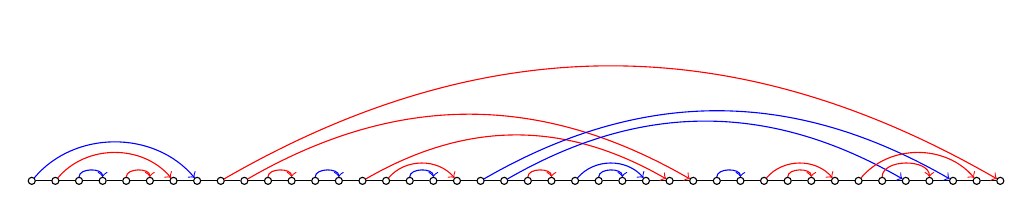
\begin{tikzpicture}[-,node distance=.5cm,auto,main node/.style={circle,draw,align=center,minimum size=1.5mm},every node/.style={scale=.6}]

        \node[main node, inner sep=1pt] (A1) {};
        \node[main node, inner sep=0pt] (A2) [right of=A1] {};
        \node[main node, inner sep=0pt] (A3) [right of=A2] {};
        \node[main node, inner sep=0pt] (A4) [right of=A3] {};
        
        \node[main node, inner sep=0pt] (A5) [right of=A4] {};
        \node[main node, inner sep=0pt] (A6) [right of=A5] {};
        \node[main node, inner sep=0pt] (A7) [right of=A6] {};
        \node[main node, inner sep=0pt] (A8) [right of=A7] {};
        \node[main node, inner sep=0pt] (A9) [right of=A8] {};
        \node[main node, inner sep=0pt] (A10) [right of=A9] {};
        \node[main node, inner sep=0pt] (A11) [right of=A10] {};
        \node[main node, inner sep=0pt] (A12) [right of=A11] {};
        \node[main node, inner sep=0pt] (A13) [right of=A12] {};
        \node[main node, inner sep=0pt] (A14) [right of=A13] {};
        \node[main node, inner sep=0pt] (A15) [right of=A14] {};
        \node[main node, inner sep=0pt] (A16) [right of=A15] {};
        \node[main node, inner sep=0pt] (A17) [right of=A16] {};
        
        \node[main node, inner sep=0pt] (A18) [right of=A17] {};
        \node[main node, inner sep=0pt] (A19) [right of=A18] {};
        \node[main node, inner sep=0pt] (A20) [right of=A19] {};
        \node[main node, inner sep=0pt] (A21) [right of=A20] {};
        \node[main node, inner sep=0pt] (A22) [right of=A21] {};
        \node[main node, inner sep=0pt] (A23) [right of=A22] {};
        \node[main node, inner sep=0pt] (A24) [right of=A23] {};
        \node[main node, inner sep=0pt] (A25) [right of=A24] {};
        \node[main node, inner sep=0pt] (A26) [right of=A25] {};
        \node[main node, inner sep=0pt] (A27) [right of=A26] {};
        \node[main node, inner sep=0pt] (A28) [right of=A27] {};
        \node[main node, inner sep=0pt] (A29) [right of=A28] {};
        \node[main node, inner sep=0pt] (A30) [right of=A29] {};
        \node[main node, inner sep=0pt] (A31) [right of=A30] {};
        \node[main node, inner sep=0pt] (A32) [right of=A31] {};
        
        
        \node[main node, inner sep=0pt] (A33) [right of=A32] {};
        \node[main node, inner sep=0pt] (A34) [right of=A33] {};
        \node[main node, inner sep=0pt] (A35) [right of=A34] {};
        \node[main node, inner sep=0pt] (A36) [right of=A35] {};
        \node[main node, inner sep=0pt] (A37) [right of=A36] {};
        \node[main node, inner sep=0pt] (A38) [right of=A37] {};
        \node[main node, inner sep=0pt] (A39) [right of=A38] {};
        \node[main node, inner sep=0pt] (A40) [right of=A39] {};
        \node[main node, inner sep=0pt] (A41) [right of=A40] {};
        \node[main node, inner sep=0pt] (A42) [right of=A41] {};
       
        %the straight lines
        
        \path (A1) edge node [right] {} (A2);
        \path (A2) edge node [right] {} (A3);
        \path (A3) edge node [right] {} (A4);
        
        \path (A4) edge node [right] {} (A5);
        \path (A5) edge node [right] {} (A6);
        \path (A6) edge node [right] {} (A7);
        \path (A7) edge node [right] {} (A8);
        \path (A8) edge node [right] {} (A9);
        \path (A9) edge node [right] {} (A10);
        \path (A10) edge node [right] {} (A11);
        \path (A11) edge node [right] {} (A12);
        \path (A12) edge node [right] {} (A13);
        \path (A13) edge node [right] {} (A14);
        \path (A14) edge node [right] {} (A15);
        \path (A15) edge node [right] {} (A16);
        \path (A16) edge node [right] {} (A17);
        \path (A17) edge node [right] {} (A18);
        \path (A18) edge node [right] {} (A19);
        \path (A19) edge node [right] {} (A20);
        \path (A20) edge node [right] {} (A21);
        \path (A21) edge node [right] {} (A22);
        \path (A22) edge node [right] {} (A23);
        \path (A23) edge node [right] {} (A24);
        \path (A24) edge node [right] {} (A25);
        \path (A25) edge node [right] {} (A26);
        \path (A26) edge node [right] {} (A27);
        \path (A27) edge node [right] {} (A28);
        \path (A28) edge node [right] {} (A29);
        \path (A29) edge node [right] {} (A30);
        \path (A30) edge node [right] {} (A31);
        \path (A31) edge node [right] {} (A32);
        
        \path (A32) edge node [right] {} (A33);
        \path (A33) edge node [right] {} (A34);
        \path (A34) edge node [right] {} (A35);
        \path (A35) edge node [right] {} (A36);
        \path (A36) edge node [right] {} (A37);
        \path (A37) edge node [right] {} (A38);
        \path (A38) edge node [right] {} (A39);
        \path (A39) edge node [right] {} (A40);
        \path (A40) edge node [right] {} (A41);
        \path (A41) edge node [right] {} (A42);
        
    %the curved lines
%        \path[->] (A2) edge [bend left=45,cyan] node {} (A6);
%        \path[->] (A2) edge [bend left=45,cyan] node {} (A11);
%        \path[->] (A2) edge [bend left=45,cyan] node {} (A13);
%        
%        \path[->] (A14) edge [bend left=45,cyan] node {} (A17);
%        \path[->] (A14) edge [bend left=45,cyan] node {} (A19);
%        \path[->] (A14) edge [bend left=45,cyan] node {} (A22);
%        
%        \path[->] (A25) edge [bend left=45,cyan] node {} (A27);
%        \path[->] (A25) edge [bend left=45,cyan] node {} (A29);
%        \path[->] (A25) edge [bend left=45,cyan] node {} (A32);
%        
%        
%         \path[->] (A4) edge [bend left=45,green!60] node {} (A8);
%        \path[->] (A4) edge [bend left=45,green!60] node {} (A12);
%        \path[->] (A4) edge [bend left=45,green!60] node {} (A16);
%        \path[->] (A4) edge [bend left=45,green!60] node {} (A19);
%        
%        
%         \path[->] (A20) edge [bend left=45,green!60] node {} (A23);
%        \path[->] (A20) edge [bend left=45,green!60] node {} (A25);
%        \path[->] (A20) edge [bend left=45,green!60] node {} (A31);
        
        
        %first WS
        \path[->] (A1) edge [bend left=50,blue] node {} (A8);
        \path[->] (A2) edge [bend left=50,red] node {} (A7);
        \path[->] (A3) edge [bend left=90,blue] node {} (A4);
        \path[->] (A5) edge [bend left=90,red] node {} (A6);
        %second stack edges
        
        \path[->] (A9) edge [bend left=30,red] node {} (A42);
        \path[->] (A10) edge [bend left=30,red] node {} (A29);
        \path[->] (A11) edge [bend left=90,red] node {} (A12);
        \path[->] (A13) edge [bend left=90,blue] node {} (A14);
        \path[->] (A15) edge [bend left=30,red] node {} (A28);
        \path[->] (A16) edge [bend left=50,red] node {} (A19);
        \path[->] (A17) edge [bend left=90,blue] node {} (A18);
        \path[->] (A20) edge [bend left=30,blue] node {} (A40);
        \path[->] (A21) edge [bend left=30,blue] node {} (A38);
        \path[->] (A22) edge [bend left=90,red] node {} (A23);
        \path[->] (A24) edge [bend left=50,blue] node {} (A27);
        \path[->] (A25) edge [bend left=90,blue] node {} (A26);
        \path[->] (A30) edge [bend left=90,blue] node {} (A31);
        \path[->] (A32) edge [bend left=50,red] node {} (A35);
        \path[->] (A33) edge [bend left=90,red] node {} (A34);
        \path[->] (A36) edge [bend left=50,red] node {} (A41);
        \path[->] (A37) edge [bend left=90,red] node {} (A39);
        
        %third stack edges
        
%        \path[->] (A6) edge [bend left=30,black] node {} (A21);
%        \path[->] (A11) edge [bend left=30,black] node {} (A17);
%        \path[->] (A15) edge [bend left=30,black] node {} (A18);
%        \path[->] (A19) edge [bend left=30,black] node {} (A22);
%        
%        % last stack edges 
%        \path[->] (A8) edge [bend left=30,violet] node {} (A30);
%        \path[->] (A13) edge [bend left=30,violet] node {} (A28);
%        \path[->] (A16) edge [bend left=30,violet] node {} (A26);
%        \path[->] (A20) edge [bend left=30,violet] node {} (A24);
        \end{tikzpicture}
        }
        \end{figure}
 \pause
  \begin{figure}[b]
\scalebox{.7}{
\begin{tikzpicture}[->,thick]
\tikzset
  {dest/.style={circle,draw,minimum width=0.005mm,inner sep=0mm}}
 %\node[state, draw=white,initial,initial text={}] (s) at (-1.8,0) {$s_0$};
 \draw (-1,-0.3) rectangle (1,0.5);
 \draw[->] (-1.3,0) -- (-1.05,0);
 \node[dest] (s0) at (-.9,0) {};
  \node[dest] (s1) at (-.7,0) {};
 \node[dest] (s2) at (-0.5,0) {};
  \node[dest] (s3) at (-0.1,0) {};
 \node[dest] (s6) at (0.5,0) {};
 \node[dest] (s7) at (.1,0) {};
  \node[dest] (s4) at (0.7,0) {};
 \node[dest] (s5) at (0.9,0) {};
 \node[dest] (s5) at (0.9,0) {};
 % \node[dest,draw=white] (l1) at (0.1,-0.6) {$ws_1$};
\put(0.1,-16.9){$ws_1$};
 \path(s1) edge[draw=red,bend left=50] node[above] {} node{}(s4);
\path(s2) edge[draw=blue,bend left=60] node[above] {} node{}(s3);
\path(s0) edge[draw=blue,bend left=50] node[above] {} node{}(s5);
 \path(s7) edge[draw=red,bend left=90] node[above] {} node{}(s6);
\draw[->] (1,0) -- (1.2,0);
\node[circle,dashed,minimum width=0.05mm,inner sep=0.5mm] (p1) at (1.35,0) {$\textcolor{red}{\downarrow_1}$};
\node[circle,dashed,minimum width=0.05mm, inner sep=0.5mm] (p2) at (1.8,0) {$\textcolor{red}{\downarrow_1}$};
\draw[->] (1.45,0) -- (1.65,0);

 \draw (2.15,-0.2) rectangle (2.95,0.3);
 \draw[->] (1.95,0) -- (2.15,0);
 \node[dest] (t0) at (2.21,0) {};
  \node[dest] (t1) at (2.5,0) {};
 \node[dest] (t2) at (2.65,0) {};
  \node[dest] (t3) at (2.85,0) {};
  \path(t0) edge[draw=red,bend left=50] node[above] {} node{}(t1);
\path(t2) edge[draw=blue,bend left=60] node[above] {} node{}(t3);
\node[circle,dashed,minimum width=0.05mm, inner sep=0.5mm] (p3) at (3.35,0) {$\textcolor{red}{\downarrow_1}$};
 \node[dest,draw=white] (dum2) at (4.5,0) {};
\put(66,-16.9){$ws_2$};
\put(110,-16.9){$ws_3$};
\put(170,-16.9){$ws_4$};

\draw[->] (2.95,0) -- (3.2,0);
\draw (3.7,-0.2) rectangle (4.5,0.3);
 \draw[->] (3.49,0) -- (3.7,0);
 \node[dest] (r0) at (3.8,0) {};
  \node[dest] (r1) at (4,0) {};
 \node[dest] (r2) at (4.2,0) {};
  \node[dest] (r3) at (4.4,0) {};
  \path(r0) edge[draw=red,bend left=50] node[above] {} node{}(r3);
\path(r1) edge[draw=blue,bend left=60] node[above] {} node{}(r2);

\node[circle,dashed,minimum width=0.05mm, inner sep=0.5mm] (p4) at (4.85,0) {$\textcolor{blue}{\downarrow_2}$};
\node[circle,dashed,minimum width=0.05mm, inner sep=0.5mm] (p5) at (5.35,0) {$\textcolor{blue}{\downarrow_2}$};
\draw[->] (4.5,0) -- (4.7,0);
 \draw[->] (4.95,0) -- (5.2,0);
 
\draw (5.65,-0.2) rectangle (6.8,0.3);
 \draw[->] (5.45,0) -- (5.65,0);
 \node[dest] (q0) at (5.75,0) {};
  \node[dest] (q1) at (5.95,0) {};
 \node[dest] (q2) at (6.15,0) {};
 \node[dest] (q3) at (6.35,0) {};
   \node[dest] (q4) at (6.5,0) {};
 \node[dest] (q5) at (6.7,0) {};
   \path(q0) edge[draw=red,bend left=50] node[above] {} node{}(q1);
\path(q2) edge[draw=blue,bend left=60] node[above] {} node{}(q5);
\path(q3) edge[draw=blue,bend left=60] node[above] {} node{}(q4);

\node[circle,dashed,minimum width=0.05mm, inner sep=0.5mm] (p9) at (7.15,0) {$\textcolor{red}{\uparrow_1}$};
\node[circle,dashed,minimum width=0.05mm, inner sep=0.5mm] (p9) at (7.65,0) {$\textcolor{red}{\uparrow_1}$};
\put(240,-16.9){$ws_5$};
\node[dest,draw=white] (dum5) at (6.95,0) {};
\node[dest,draw=white] (dum6) at (9.1,0) {};
%\node[fill=green!70, rectangle, inner sep=0.5, fill opacity=0.2,fit=(dum5)(p9)(dum6)](H){};


 \draw[->] (6.8,0) -- (7,0);
\draw[->] (7.3,0) -- (7.5,0);

\draw (8,-0.2) rectangle (9.2,0.3);
 \draw[->] (7.75,0) -- (8,0);
 \node[dest] (d0) at (8.1,0) {};
  \node[dest] (d1) at (8.3,0) {};
 \node[dest] (d2) at (8.5,0) {};
 \node[dest] (d3) at (8.7,0) {};
   \node[dest] (d4) at (8.9,0) {};
 \node[dest] (d5) at (9.1,0) {};
   \path(d0) edge[draw=blue,bend left=50] node[above] {} node{}(d1);
\path(d2) edge[draw=red,bend left=60] node[above] {} node{}(d5);
\path(d3) edge[draw=red,bend left=60] node[above] {} node{}(d4);


\node[circle,dashed,minimum width=0.05mm, inner sep=0.5mm] (p6) at (9.5,0) {$\textcolor{red}{\downarrow_1}$};
\node[circle,dashed,minimum width=0.05mm, inner sep=0.5mm] (p7) at (9.95,0) {$\textcolor{red}{\downarrow_1}$};

\node[circle,dashed,minimum width=0.05mm, inner sep=0.5mm] (p8) at (10.5,0) {$\textcolor{blue}{\uparrow_2}$};
\node[circle,dashed,minimum width=0.05mm, inner sep=0.5mm] (p9) at (10.9,0) {$\textcolor{red}{\uparrow_1}$};
\node[circle,dashed,minimum width=0.05mm, inner sep=0.5mm] (p10) at (11.3,0) {$\textcolor{blue}{\uparrow_2}$};
\node[circle,dashed,minimum width=0.05mm, inner sep=0.5mm] (p9) at (11.7,0) {$\textcolor{red}{\uparrow_1}$};
\node[circle,dashed,minimum width=0.05mm, inner sep=0.5mm] (p9) at (12.1,0) {$\textcolor{red}{\uparrow_1}$};
%\node[circle,dashed,minimum width=0.05mm, inner sep=0.5mm] (p10) at (12.6,0) {$s_f$};
\node[dest,draw=white] (dum7) at (11.6,-.2) {};
\node[dest,draw=white] (dum8) at (12.21,0.2) {};

%\node[fill=green!70, rectangle, inner sep=0.5, fill opacity=0.2,fit=(dum7)(dum8)](H11){};

\draw[->] (9.2,0)--(9.38,0);
\draw[->] (9.6,0)--(9.78,0);
\draw[->] (10.05,0)--(10.28,0);
 \draw[->] (10.55,0)--(10.73,0);
 \draw[->] (10.95,0)--(11.15,0);
\draw[->] (11.38,0)--(11.55,0);
\draw[->] (11.77,0)--(11.95,0);
\draw[->] (12.15,0)--(12.35,0);

\node[fill=red!50, rectangle, inner sep=0.5, fill opacity=0.2,fit= (p1)(dum2)](H1){};
\node[dest,draw=white] (dum3) at (6.76,0) {};

\node[fill=blue!50, rectangle, inner sep=0.5, fill opacity=0.2,fit= (p4)(dum3)](H1){};

\node[dest,draw=white] (dum4) at (9.8,0) {};

\node[fill=red!50, rectangle, inner sep=0.5, fill opacity=0.2,fit=
(p6)(p7)](H1){};

\end{tikzpicture}
}
 % \caption{A run $\sigma$ of MPDA, $\downarrow^{i}$ and $\uparrow^{i}$ represents push at stack
%    $i$ and   pop at stack $i$ respectively
% % The green  patches are pop-holes of the red stack.
% }
\label{run:holes1}
\end{figure}

%%% Local Variables:
%%% mode: latex
%%% TeX-master: "main"
%%% End:

   % \vspace{-1cm}
  
   % Every run of a \mpda{} is made of three basic blocks 
   \begin{itemize}[<+->]
   \item Well-nested sequence ($ws_{j}$) \textcolor{blue}{ can be
       $\varepsilon$}
     \item Pushes not part of a well-nested sequence (represented as
       $\downarrow_i$ )
        \item Matching pops that are matched with $\downarrow_i$ ( represented
          as$\uparrow_{i}$) 
     \item An atomic-i-segment of stack $i$ is a push $\downarrow_i$ followed by a
       well-nested sequence $ws_{j}$.
   \item An i-segment is the concatenation of multiple
     atomic-i-segments 
   
   \end{itemize}
\end{frame}
% %%%%%%%%%%%%%%%
 \begin{frame}[t]{ Segments and holes}
   \begin{figure}[b]
\scalebox{.7}{
\begin{tikzpicture}[->,thick]
\tikzset
  {dest/.style={circle,draw,minimum width=0.005mm,inner sep=0mm}}
 %\node[state, draw=white,initial,initial text={}] (s) at (-1.8,0) {$s_0$};
 \draw (-1,-0.3) rectangle (1,0.5);
 \draw[->] (-1.3,0) -- (-1.05,0);
 \node[dest] (s0) at (-.9,0) {};
  \node[dest] (s1) at (-.7,0) {};
 \node[dest] (s2) at (-0.5,0) {};
  \node[dest] (s3) at (-0.1,0) {};
 \node[dest] (s6) at (0.5,0) {};
 \node[dest] (s7) at (.1,0) {};
  \node[dest] (s4) at (0.7,0) {};
 \node[dest] (s5) at (0.9,0) {};
 \node[dest] (s5) at (0.9,0) {};
 % \node[dest,draw=white] (l1) at (0.1,-0.6) {$ws_1$};
\put(0.1,-16.9){$ws_1$};
 \path(s1) edge[draw=red,bend left=50] node[above] {} node{}(s4);
\path(s2) edge[draw=blue,bend left=60] node[above] {} node{}(s3);
\path(s0) edge[draw=blue,bend left=50] node[above] {} node{}(s5);
 \path(s7) edge[draw=red,bend left=90] node[above] {} node{}(s6);
\draw[->] (1,0) -- (1.2,0);
\node[circle,dashed,minimum width=0.05mm,inner sep=0.5mm] (p1) at (1.35,0) {$\textcolor{red}{\downarrow_1}$};
\node[circle,dashed,minimum width=0.05mm, inner sep=0.5mm] (p2) at (1.8,0) {$\textcolor{red}{\downarrow_1}$};
\draw[->] (1.45,0) -- (1.65,0);

 \draw (2.15,-0.2) rectangle (2.95,0.3);
 \draw[->] (1.95,0) -- (2.15,0);
 \node[dest] (t0) at (2.21,0) {};
  \node[dest] (t1) at (2.5,0) {};
 \node[dest] (t2) at (2.65,0) {};
  \node[dest] (t3) at (2.85,0) {};
  \path(t0) edge[draw=red,bend left=50] node[above] {} node{}(t1);
\path(t2) edge[draw=blue,bend left=60] node[above] {} node{}(t3);
\node[circle,dashed,minimum width=0.05mm, inner sep=0.5mm] (p3) at (3.35,0) {$\textcolor{red}{\downarrow_1}$};
 \node[dest,draw=white] (dum2) at (4.5,0) {};
\put(66,-16.9){$ws_2$};
\put(110,-16.9){$ws_3$};
\put(170,-16.9){$ws_4$};

\draw[->] (2.95,0) -- (3.2,0);
\draw (3.7,-0.2) rectangle (4.5,0.3);
 \draw[->] (3.49,0) -- (3.7,0);
 \node[dest] (r0) at (3.8,0) {};
  \node[dest] (r1) at (4,0) {};
 \node[dest] (r2) at (4.2,0) {};
  \node[dest] (r3) at (4.4,0) {};
  \path(r0) edge[draw=red,bend left=50] node[above] {} node{}(r3);
\path(r1) edge[draw=blue,bend left=60] node[above] {} node{}(r2);

\node[circle,dashed,minimum width=0.05mm, inner sep=0.5mm] (p4) at (4.85,0) {$\textcolor{blue}{\downarrow_2}$};
\node[circle,dashed,minimum width=0.05mm, inner sep=0.5mm] (p5) at (5.35,0) {$\textcolor{blue}{\downarrow_2}$};
\draw[->] (4.5,0) -- (4.7,0);
 \draw[->] (4.95,0) -- (5.2,0);
 
\draw (5.65,-0.2) rectangle (6.8,0.3);
 \draw[->] (5.45,0) -- (5.65,0);
 \node[dest] (q0) at (5.75,0) {};
  \node[dest] (q1) at (5.95,0) {};
 \node[dest] (q2) at (6.15,0) {};
 \node[dest] (q3) at (6.35,0) {};
   \node[dest] (q4) at (6.5,0) {};
 \node[dest] (q5) at (6.7,0) {};
   \path(q0) edge[draw=red,bend left=50] node[above] {} node{}(q1);
\path(q2) edge[draw=blue,bend left=60] node[above] {} node{}(q5);
\path(q3) edge[draw=blue,bend left=60] node[above] {} node{}(q4);

\node[circle,dashed,minimum width=0.05mm, inner sep=0.5mm] (p9) at (7.15,0) {$\textcolor{red}{\uparrow_1}$};
\node[circle,dashed,minimum width=0.05mm, inner sep=0.5mm] (p9) at (7.65,0) {$\textcolor{red}{\uparrow_1}$};
\put(240,-16.9){$ws_5$};
\node[dest,draw=white] (dum5) at (6.95,0) {};
\node[dest,draw=white] (dum6) at (9.1,0) {};
%\node[fill=green!70, rectangle, inner sep=0.5, fill opacity=0.2,fit=(dum5)(p9)(dum6)](H){};


 \draw[->] (6.8,0) -- (7,0);
\draw[->] (7.3,0) -- (7.5,0);

\draw (8,-0.2) rectangle (9.2,0.3);
 \draw[->] (7.75,0) -- (8,0);
 \node[dest] (d0) at (8.1,0) {};
  \node[dest] (d1) at (8.3,0) {};
 \node[dest] (d2) at (8.5,0) {};
 \node[dest] (d3) at (8.7,0) {};
   \node[dest] (d4) at (8.9,0) {};
 \node[dest] (d5) at (9.1,0) {};
   \path(d0) edge[draw=blue,bend left=50] node[above] {} node{}(d1);
\path(d2) edge[draw=red,bend left=60] node[above] {} node{}(d5);
\path(d3) edge[draw=red,bend left=60] node[above] {} node{}(d4);


\node[circle,dashed,minimum width=0.05mm, inner sep=0.5mm] (p6) at (9.5,0) {$\textcolor{red}{\downarrow_1}$};
\node[circle,dashed,minimum width=0.05mm, inner sep=0.5mm] (p7) at (9.95,0) {$\textcolor{red}{\downarrow_1}$};

\node[circle,dashed,minimum width=0.05mm, inner sep=0.5mm] (p8) at (10.5,0) {$\textcolor{blue}{\uparrow_2}$};
\node[circle,dashed,minimum width=0.05mm, inner sep=0.5mm] (p9) at (10.9,0) {$\textcolor{red}{\uparrow_1}$};
\node[circle,dashed,minimum width=0.05mm, inner sep=0.5mm] (p10) at (11.3,0) {$\textcolor{blue}{\uparrow_2}$};
\node[circle,dashed,minimum width=0.05mm, inner sep=0.5mm] (p9) at (11.7,0) {$\textcolor{red}{\uparrow_1}$};
\node[circle,dashed,minimum width=0.05mm, inner sep=0.5mm] (p9) at (12.1,0) {$\textcolor{red}{\uparrow_1}$};
%\node[circle,dashed,minimum width=0.05mm, inner sep=0.5mm] (p10) at (12.6,0) {$s_f$};
\node[dest,draw=white] (dum7) at (11.6,-.2) {};
\node[dest,draw=white] (dum8) at (12.21,0.2) {};

%\node[fill=green!70, rectangle, inner sep=0.5, fill opacity=0.2,fit=(dum7)(dum8)](H11){};

\draw[->] (9.2,0)--(9.38,0);
\draw[->] (9.6,0)--(9.78,0);
\draw[->] (10.05,0)--(10.28,0);
 \draw[->] (10.55,0)--(10.73,0);
 \draw[->] (10.95,0)--(11.15,0);
\draw[->] (11.38,0)--(11.55,0);
\draw[->] (11.77,0)--(11.95,0);
\draw[->] (12.15,0)--(12.35,0);

\node[fill=red!50, rectangle, inner sep=0.5, fill opacity=0.2,fit= (p1)(dum2)](H1){};
\node[dest,draw=white] (dum3) at (6.76,0) {};

\node[fill=blue!50, rectangle, inner sep=0.5, fill opacity=0.2,fit= (p4)(dum3)](H1){};

\node[dest,draw=white] (dum4) at (9.8,0) {};

\node[fill=red!50, rectangle, inner sep=0.5, fill opacity=0.2,fit=
(p6)(p7)](H1){};

\end{tikzpicture}
}
 % \caption{A run $\sigma$ of MPDA, $\downarrow^{i}$ and $\uparrow^{i}$ represents push at stack
%    $i$ and   pop at stack $i$ respectively
% % The green  patches are pop-holes of the red stack.
% }
\label{run:holes1}
\end{figure}

%%% Local Variables:
%%% mode: latex
%%% TeX-master: "main"
%%% End:
 
%   \vspace{-1cm}
   \begin{itemize}[<+->]
 
   \item \textbf{Pending-push($\downarrow_{i}$)} of stack $i$ (w.r.t
     a position \textcolor{red}{n}) \\
 \textcolor{red}{  \texttt{No matching pop prior  $n$ }}
     
  \item \textbf{An i-segment} is open if its first push transitions are
    pending
    \item \textbf{An i-hole} in a run is the maximal factor that is an open
      i-segment 
     \item  We denote by $\nbholes{\sigma}$ the number of holes in a run $\sigma$

      
    
     
  
     
   \end{itemize}
 \end{frame}
% %%%%%%%%%%%%%%%%%%%%%%
 \begin{frame}{\textbf{Hole} Bounded runs of \mpda{}}
 
     \begin{figure}[b]
\scalebox{.7}{
\begin{tikzpicture}[->,thick]
\tikzset
  {dest/.style={circle,draw,minimum width=0.005mm,inner sep=0mm}}
 %\node[state, draw=white,initial,initial text={}] (s) at (-1.8,0) {$s_0$};
 \draw (-1,-0.3) rectangle (1,0.5);
 \draw[->] (-1.3,0) -- (-1.05,0);
 \node[dest] (s0) at (-.9,0) {};
  \node[dest] (s1) at (-.7,0) {};
 \node[dest] (s2) at (-0.5,0) {};
  \node[dest] (s3) at (-0.1,0) {};
 \node[dest] (s6) at (0.5,0) {};
 \node[dest] (s7) at (.1,0) {};
  \node[dest] (s4) at (0.7,0) {};
 \node[dest] (s5) at (0.9,0) {};
 \node[dest] (s5) at (0.9,0) {};
 % \node[dest,draw=white] (l1) at (0.1,-0.6) {$ws_1$};
\put(0.1,-16.9){$ws_1$};
 \path(s1) edge[draw=red,bend left=50] node[above] {} node{}(s4);
\path(s2) edge[draw=blue,bend left=60] node[above] {} node{}(s3);
\path(s0) edge[draw=blue,bend left=50] node[above] {} node{}(s5);
 \path(s7) edge[draw=red,bend left=90] node[above] {} node{}(s6);
\draw[->] (1,0) -- (1.2,0);
\node[circle,dashed,minimum width=0.05mm,inner sep=0.5mm] (p1) at (1.35,0) {$\textcolor{red}{\downarrow_1}$};
\node[circle,dashed,minimum width=0.05mm, inner sep=0.5mm] (p2) at (1.8,0) {$\textcolor{red}{\downarrow_1}$};
\draw[->] (1.45,0) -- (1.65,0);

 \draw (2.15,-0.2) rectangle (2.95,0.3);
 \draw[->] (1.95,0) -- (2.15,0);
 \node[dest] (t0) at (2.21,0) {};
  \node[dest] (t1) at (2.5,0) {};
 \node[dest] (t2) at (2.65,0) {};
  \node[dest] (t3) at (2.85,0) {};
  \path(t0) edge[draw=red,bend left=50] node[above] {} node{}(t1);
\path(t2) edge[draw=blue,bend left=60] node[above] {} node{}(t3);
\node[circle,dashed,minimum width=0.05mm, inner sep=0.5mm] (p3) at (3.35,0) {$\textcolor{red}{\downarrow_1}$};
 \node[dest,draw=white] (dum2) at (4.5,0) {};
\put(66,-16.9){$ws_2$};
\put(110,-16.9){$ws_3$};
\put(170,-16.9){$ws_4$};

\draw[->] (2.95,0) -- (3.2,0);
\draw (3.7,-0.2) rectangle (4.5,0.3);
 \draw[->] (3.49,0) -- (3.7,0);
 \node[dest] (r0) at (3.8,0) {};
  \node[dest] (r1) at (4,0) {};
 \node[dest] (r2) at (4.2,0) {};
  \node[dest] (r3) at (4.4,0) {};
  \path(r0) edge[draw=red,bend left=50] node[above] {} node{}(r3);
\path(r1) edge[draw=blue,bend left=60] node[above] {} node{}(r2);

\node[circle,dashed,minimum width=0.05mm, inner sep=0.5mm] (p4) at (4.85,0) {$\textcolor{blue}{\downarrow_2}$};
\node[circle,dashed,minimum width=0.05mm, inner sep=0.5mm] (p5) at (5.35,0) {$\textcolor{blue}{\downarrow_2}$};
\draw[->] (4.5,0) -- (4.7,0);
 \draw[->] (4.95,0) -- (5.2,0);
 
\draw (5.65,-0.2) rectangle (6.8,0.3);
 \draw[->] (5.45,0) -- (5.65,0);
 \node[dest] (q0) at (5.75,0) {};
  \node[dest] (q1) at (5.95,0) {};
 \node[dest] (q2) at (6.15,0) {};
 \node[dest] (q3) at (6.35,0) {};
   \node[dest] (q4) at (6.5,0) {};
 \node[dest] (q5) at (6.7,0) {};
   \path(q0) edge[draw=red,bend left=50] node[above] {} node{}(q1);
\path(q2) edge[draw=blue,bend left=60] node[above] {} node{}(q5);
\path(q3) edge[draw=blue,bend left=60] node[above] {} node{}(q4);

\node[circle,dashed,minimum width=0.05mm, inner sep=0.5mm] (p9) at (7.15,0) {$\textcolor{red}{\uparrow_1}$};
\node[circle,dashed,minimum width=0.05mm, inner sep=0.5mm] (p9) at (7.65,0) {$\textcolor{red}{\uparrow_1}$};
\put(240,-16.9){$ws_5$};
\node[dest,draw=white] (dum5) at (6.95,0) {};
\node[dest,draw=white] (dum6) at (9.1,0) {};
%\node[fill=green!70, rectangle, inner sep=0.5, fill opacity=0.2,fit=(dum5)(p9)(dum6)](H){};


 \draw[->] (6.8,0) -- (7,0);
\draw[->] (7.3,0) -- (7.5,0);

\draw (8,-0.2) rectangle (9.2,0.3);
 \draw[->] (7.75,0) -- (8,0);
 \node[dest] (d0) at (8.1,0) {};
  \node[dest] (d1) at (8.3,0) {};
 \node[dest] (d2) at (8.5,0) {};
 \node[dest] (d3) at (8.7,0) {};
   \node[dest] (d4) at (8.9,0) {};
 \node[dest] (d5) at (9.1,0) {};
   \path(d0) edge[draw=blue,bend left=50] node[above] {} node{}(d1);
\path(d2) edge[draw=red,bend left=60] node[above] {} node{}(d5);
\path(d3) edge[draw=red,bend left=60] node[above] {} node{}(d4);


\node[circle,dashed,minimum width=0.05mm, inner sep=0.5mm] (p6) at (9.5,0) {$\textcolor{red}{\downarrow_1}$};
\node[circle,dashed,minimum width=0.05mm, inner sep=0.5mm] (p7) at (9.95,0) {$\textcolor{red}{\downarrow_1}$};

\node[circle,dashed,minimum width=0.05mm, inner sep=0.5mm] (p8) at (10.5,0) {$\textcolor{blue}{\uparrow_2}$};
\node[circle,dashed,minimum width=0.05mm, inner sep=0.5mm] (p9) at (10.9,0) {$\textcolor{red}{\uparrow_1}$};
\node[circle,dashed,minimum width=0.05mm, inner sep=0.5mm] (p10) at (11.3,0) {$\textcolor{blue}{\uparrow_2}$};
\node[circle,dashed,minimum width=0.05mm, inner sep=0.5mm] (p9) at (11.7,0) {$\textcolor{red}{\uparrow_1}$};
\node[circle,dashed,minimum width=0.05mm, inner sep=0.5mm] (p9) at (12.1,0) {$\textcolor{red}{\uparrow_1}$};
%\node[circle,dashed,minimum width=0.05mm, inner sep=0.5mm] (p10) at (12.6,0) {$s_f$};
\node[dest,draw=white] (dum7) at (11.6,-.2) {};
\node[dest,draw=white] (dum8) at (12.21,0.2) {};

%\node[fill=green!70, rectangle, inner sep=0.5, fill opacity=0.2,fit=(dum7)(dum8)](H11){};

\draw[->] (9.2,0)--(9.38,0);
\draw[->] (9.6,0)--(9.78,0);
\draw[->] (10.05,0)--(10.28,0);
 \draw[->] (10.55,0)--(10.73,0);
 \draw[->] (10.95,0)--(11.15,0);
\draw[->] (11.38,0)--(11.55,0);
\draw[->] (11.77,0)--(11.95,0);
\draw[->] (12.15,0)--(12.35,0);

\node[fill=red!50, rectangle, inner sep=0.5, fill opacity=0.2,fit= (p1)(dum2)](H1){};
\node[dest,draw=white] (dum3) at (6.76,0) {};

\node[fill=blue!50, rectangle, inner sep=0.5, fill opacity=0.2,fit= (p4)(dum3)](H1){};

\node[dest,draw=white] (dum4) at (9.8,0) {};

\node[fill=red!50, rectangle, inner sep=0.5, fill opacity=0.2,fit=
(p6)(p7)](H1){};

\end{tikzpicture}
}
 % \caption{A run $\sigma$ of MPDA, $\downarrow^{i}$ and $\uparrow^{i}$ represents push at stack
%    $i$ and   pop at stack $i$ respectively
% % The green  patches are pop-holes of the red stack.
% }
\label{run:holes1}
\end{figure}

%%% Local Variables:
%%% mode: latex
%%% TeX-master: "main"
%%% End:

   \begin{definition}
     A run $\sigma$ is said to be \textcolor{red}{\textbf{$K$-hole}}
     bounded if $\nbholes{\sigma} \leq K$, for $K\in \mathbb{N}$.
   \end{definition}
    \vspace{1cm} In \textcolor{red}{\textbf{hole} bounded}
   reachability of \mpda{} we only search for a
   \textcolor{red}{\textbf{K-hole}} bounded accepting run of \mpda{}
   where, \textbf{K}$\in \mathbb{N}$.
 
    
 \end{frame}

  %%%%%%%%%%%%%%%%%%%%%%%
%\subsection{Contributions}
\begin{frame}{Hierarchy of Under-approximations}

   
\begin{figure}[h!]
  \centering \scalebox{0.8}{
    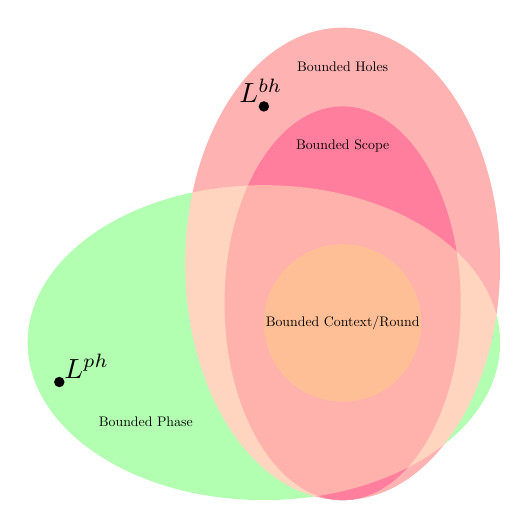
\begin{tikzpicture}
      \begin{scope}[blend group = soft light]
        \fill[red!30!white] ( 1,0) ellipse (2 and 3);
        \fill[green!30!white] (0,-1) ellipse (3 and 2);
        \fill[blue!30!red] (1,-.5) ellipse ( 1.5 and 2.5);
        \fill[blue!30!green] (1,-.75) circle (1);
        
      \end{scope}
      \node[circle,fill,color=black,scale=.4] at ( 90:2) {};
      \node[circle,fill,color=black,scale=.4] at ( 210:3) {}; \node at
      (210:2.6) {$L^{ph}$}; \node at (91:2.2) {$L^{bh}$};
      \node[scale=.5] at (1,2.5) {Bounded Holes}; \node[scale=.5] at (
      1,1.5) {Bounded Scope}; \node[scale=.5] at (1,-.75) {Bounded
        Context/Round}; \node[scale=.5] at (-1.5,-2) {Bounded Phase};
      
    \end{tikzpicture}
  }
\end{figure}

 $L^{ph} = \{(ab)^nc^nd^n| n \in \mathbb{N}\} $
 $L^{bh} = \{a^nb^n(a^{q_1}c^{q_1+1}b^{q'_1}d^{q'_1+1}\cdots  a^{q_n}c^{q_n+1}b^{q'_n}d^{q'_n+1})\mid n ,q_i,q'_i \in \mathbb{N}$
\end{frame}
%%%%%%%%%%%%%%%%%%%   5
\begin{frame}{Algorithm  to Solve Hole bounded reachability}
  \textbf{Question: } Given a MPDA and a bound $K\in \mathbb{N}$ does
  there exists a $K$-hole bounded run that reaches a target state from
  the initial state?
  
  \begin{itemize}
  \item Algorithm
    \begin{itemize}
  \item Uses fixed-point computation 
  \item Guided BFS exploration
    \item Witness generation
  \end{itemize}
\end{itemize}
\end{frame}
%%%%%%%%%%%%%%%%%
\begin{frame}[t]{Steps of the Algorithm}
  We divide the algorithm in two parts,
  \begin{enumerate}[<+->]
  \item Fixed-point Computation and Memoization\\
    \only<1>{\textcolor{red}{\texttt{Precomputes well nested runs ($ws$),
        atomic open-hole $(\downarrow_{i}ws)$, and open-hole
        $(\downarrow_{i}ws)^{+}$.}}}
  \item On-The-Fly guided Breadth First Search (BFS) Exploration
    \only<2>{\textcolor{red}{\texttt{Which solves hole bounded reachability
        for \mpda{}}}}
  \end{enumerate}
\end{frame}

  %%%%%%%%%%%%%%%%%%%
      \begin{frame}{Computing Well-Nested Sequences}
        \begin{center}
        \begin{tikzpicture}[overlay, on grid, scale=0.5, every node/.style={scale=0.5},]
         \only<1->{ \node[state] at (-6,0) (q_1)  {$s_i$};}
          \only<1-3>{\node[state, right=2cm of q_1] (q_2) {$s_j$};}
         \only<2-3>{ \node[state, right=2cm of q_2] (q_3) {$s_k$};}
        \only<3->{  \node[state, right=2cm of q_3] (q_4) {$s_l$};}
         \only<1-3>{ \path[->] (q_1) edge  node [above, align=left]
          {$\downarrow^n(\alpha)$} (q_2);}
          \only<2-3>{\path[->] (q_2) edge   (q_3);}
          \only<3>{ \path[->] (q_3) edge  node [above, align=left] {$\uparrow^n(\alpha)$} (q_4);}
           \only<4->{\path[->] (q_1) edge  (q_4);}
           \only<4->{ \path[->] (q_1) edge[bend left]  node [above, align=left] {} (q_4);}
          
        \end{tikzpicture}
\end{center}
\end{frame} 
%%%%%%%%%%
  \begin{frame}{Computing Well-Nested Sequences}
      For all state $s_i$, create the following entries,
      \begin{itemize}
      \item $(s_i,s_i)$ 
        \item $(s_i,s_k)$ if $s_k$ is reachable by
          discrete transition
        \end{itemize}

        \pause
        \begin{center}  
 \scalebox{0.8}{ %\schema[close]{     
    \begin{tabular}{ c|c|c|c|c c }
        $\ddots$ & $s_j$ & $\dots$ &$s_k$& $\dots$&
                                                    \rdelim\}{4}{0cm}[$\mid
                                                    \mathcal{S}\mid$]
      \tabularnewline
        \hline
        $\vdots$ & $\vdots$ & $\dots$ &$\vdots$ &$\dots$\tabularnewline
        \hline                     
        $s_i$ & $1$ & $\dots$& $0$ & $\dots$\tabularnewline
        \hline
        $\vdots$ &  $\vdots$&$\dots$ &$\vdots$ &$\ddots$ \tabularnewline
      \end{tabular}
    }
    \end{center}
%            \scalebox{.8}{      
%         \schema[close]{
       
           
%            \begin{tabular}{ c|c|c|c|c } 
 
%            $\ddots$ & $s_i$ &$ \dots$ &$s_k$&$ \dots$ \\
%              \hline
%              $\vdots$ & $\vdots$ & $\dots$ &$\vdots$ &$\dots$\\
%              \hline
                                                       
%              $s_i$ & 1 & $\dots$& 0 &$ \dots$\\
%              \hline
%             $\vdots$ & $ \vdots$&$\dots$ &$\vdots$ &$\ddots$ \\
           
%            \end{tabular}
           
        
% }{$|\mathcal{S}|$}
% }

   %     Size of the matrix is : 
\pause


        \textcolor{red}{Transitive Closure} will give us the
        $\textbf{well-nested}$ sequences
        
      \end{frame}
      %%%%%%%%%%%%%%%
        \begin{frame}{Computing i-segments and i-holes}
        \begin{itemize}[<+->]
              \item An \textbf{i-segment} $(\downarrow^i(\alpha)ws)$ for a
               stack $i$ is a pending push($\downarrow^i$) followed by
               a maximal \textbf{well-nested} sequence($ws$)
                

              \item  We can pre-compute all possible \textbf{i-segments} by concatenating well-nested sequences after a push transition of stack $i$. 
              
              \item Assume we store this information in $M^i$
              

              \item Dropping stack alphabet and doing transitive closure
               on $M^i$ gives us information of all \textbf{i-Holes}, ($M^h_i$).
               \end{itemize}

               
                 \begin{center}
                 
    \begin{tikzpicture}[overlay,on grid,scale=0.5, every
      node/.style={scale=0.5},]
      \only<1->{ \node[state] at (-6,0) (q_1) {$s_i$};}
      \only<1->{\node[state,right=2cm of q_1] (q_2) {$s_j$};}
      \only<1->{ \node[state,right=2cm of q_2] (q_3) {$s_k$};}
      %\only<2->{ \node[state,right=2cm of q_3] (q_4) {$s_l$};}
      \only<1->{ \path[->] (q_1) edge node [above,align=left]
        {$\downarrow^i(\alpha)$} (q_2);} \only<1->{\path[->] (q_2)
        edge node [above,align=left]
        {$ws$} (q_3);}
      % \only<2>{ \path[->] (q_3) edge node
      %   [above,align=left] {$\uparrow^i(\alpha)$} (q_4);}
      % \only<3->{\path[->] (q_1) edge  node [above,align=left]
      %   {$ws'=\downarrow^i(\alpha)\cdot ws\cdot\uparrow^n(\alpha)$} (q_4);}
      %\only<5->{ \path[->]
       % (q_1) edge[bend left] node [above,align=left] {} (q_4);}
          
    \end{tikzpicture}
  \end{center}  
              \end{frame}
      %%%%%%%%%%%
      \begin{frame}{Blocks of a run of \mpda{}}
  \begin{figure}[b]
\scalebox{.7}{
\begin{tikzpicture}[->,thick]
\tikzset
  {dest/.style={circle,draw,minimum width=0.005mm,inner sep=0mm}}
 %\node[state, draw=white,initial,initial text={}] (s) at (-1.8,0) {$s_0$};
 \draw (-1,-0.3) rectangle (1,0.5);
 \draw[->] (-1.3,0) -- (-1.05,0);
 \node[dest] (s0) at (-.9,0) {};
  \node[dest] (s1) at (-.7,0) {};
 \node[dest] (s2) at (-0.5,0) {};
  \node[dest] (s3) at (-0.1,0) {};
 \node[dest] (s6) at (0.5,0) {};
 \node[dest] (s7) at (.1,0) {};
  \node[dest] (s4) at (0.7,0) {};
 \node[dest] (s5) at (0.9,0) {};
 \node[dest] (s5) at (0.9,0) {};
 % \node[dest,draw=white] (l1) at (0.1,-0.6) {$ws_1$};
\put(0.1,-16.9){$ws_1$};
 \path(s1) edge[draw=red,bend left=50] node[above] {} node{}(s4);
\path(s2) edge[draw=blue,bend left=60] node[above] {} node{}(s3);
\path(s0) edge[draw=blue,bend left=50] node[above] {} node{}(s5);
 \path(s7) edge[draw=red,bend left=90] node[above] {} node{}(s6);
\draw[->] (1,0) -- (1.2,0);
\node[circle,dashed,minimum width=0.05mm,inner sep=0.5mm] (p1) at (1.35,0) {$\textcolor{red}{\downarrow_1}$};
\node[circle,dashed,minimum width=0.05mm, inner sep=0.5mm] (p2) at (1.8,0) {$\textcolor{red}{\downarrow_1}$};
\draw[->] (1.45,0) -- (1.65,0);

 \draw (2.15,-0.2) rectangle (2.95,0.3);
 \draw[->] (1.95,0) -- (2.15,0);
 \node[dest] (t0) at (2.21,0) {};
  \node[dest] (t1) at (2.5,0) {};
 \node[dest] (t2) at (2.65,0) {};
  \node[dest] (t3) at (2.85,0) {};
  \path(t0) edge[draw=red,bend left=50] node[above] {} node{}(t1);
\path(t2) edge[draw=blue,bend left=60] node[above] {} node{}(t3);
\node[circle,dashed,minimum width=0.05mm, inner sep=0.5mm] (p3) at (3.35,0) {$\textcolor{red}{\downarrow_1}$};
 \node[dest,draw=white] (dum2) at (4.5,0) {};
\put(66,-16.9){$ws_2$};
\put(110,-16.9){$ws_3$};
\put(170,-16.9){$ws_4$};

\draw[->] (2.95,0) -- (3.2,0);
\draw (3.7,-0.2) rectangle (4.5,0.3);
 \draw[->] (3.49,0) -- (3.7,0);
 \node[dest] (r0) at (3.8,0) {};
  \node[dest] (r1) at (4,0) {};
 \node[dest] (r2) at (4.2,0) {};
  \node[dest] (r3) at (4.4,0) {};
  \path(r0) edge[draw=red,bend left=50] node[above] {} node{}(r3);
\path(r1) edge[draw=blue,bend left=60] node[above] {} node{}(r2);

\node[circle,dashed,minimum width=0.05mm, inner sep=0.5mm] (p4) at (4.85,0) {$\textcolor{blue}{\downarrow_2}$};
\node[circle,dashed,minimum width=0.05mm, inner sep=0.5mm] (p5) at (5.35,0) {$\textcolor{blue}{\downarrow_2}$};
\draw[->] (4.5,0) -- (4.7,0);
 \draw[->] (4.95,0) -- (5.2,0);
 
\draw (5.65,-0.2) rectangle (6.8,0.3);
 \draw[->] (5.45,0) -- (5.65,0);
 \node[dest] (q0) at (5.75,0) {};
  \node[dest] (q1) at (5.95,0) {};
 \node[dest] (q2) at (6.15,0) {};
 \node[dest] (q3) at (6.35,0) {};
   \node[dest] (q4) at (6.5,0) {};
 \node[dest] (q5) at (6.7,0) {};
   \path(q0) edge[draw=red,bend left=50] node[above] {} node{}(q1);
\path(q2) edge[draw=blue,bend left=60] node[above] {} node{}(q5);
\path(q3) edge[draw=blue,bend left=60] node[above] {} node{}(q4);

\node[circle,dashed,minimum width=0.05mm, inner sep=0.5mm] (p9) at (7.15,0) {$\textcolor{red}{\uparrow_1}$};
\node[circle,dashed,minimum width=0.05mm, inner sep=0.5mm] (p9) at (7.65,0) {$\textcolor{red}{\uparrow_1}$};
\put(240,-16.9){$ws_5$};
\node[dest,draw=white] (dum5) at (6.95,0) {};
\node[dest,draw=white] (dum6) at (9.1,0) {};
%\node[fill=green!70, rectangle, inner sep=0.5, fill opacity=0.2,fit=(dum5)(p9)(dum6)](H){};


 \draw[->] (6.8,0) -- (7,0);
\draw[->] (7.3,0) -- (7.5,0);

\draw (8,-0.2) rectangle (9.2,0.3);
 \draw[->] (7.75,0) -- (8,0);
 \node[dest] (d0) at (8.1,0) {};
  \node[dest] (d1) at (8.3,0) {};
 \node[dest] (d2) at (8.5,0) {};
 \node[dest] (d3) at (8.7,0) {};
   \node[dest] (d4) at (8.9,0) {};
 \node[dest] (d5) at (9.1,0) {};
   \path(d0) edge[draw=blue,bend left=50] node[above] {} node{}(d1);
\path(d2) edge[draw=red,bend left=60] node[above] {} node{}(d5);
\path(d3) edge[draw=red,bend left=60] node[above] {} node{}(d4);


\node[circle,dashed,minimum width=0.05mm, inner sep=0.5mm] (p6) at (9.5,0) {$\textcolor{red}{\downarrow_1}$};
\node[circle,dashed,minimum width=0.05mm, inner sep=0.5mm] (p7) at (9.95,0) {$\textcolor{red}{\downarrow_1}$};

\node[circle,dashed,minimum width=0.05mm, inner sep=0.5mm] (p8) at (10.5,0) {$\textcolor{blue}{\uparrow_2}$};
\node[circle,dashed,minimum width=0.05mm, inner sep=0.5mm] (p9) at (10.9,0) {$\textcolor{red}{\uparrow_1}$};
\node[circle,dashed,minimum width=0.05mm, inner sep=0.5mm] (p10) at (11.3,0) {$\textcolor{blue}{\uparrow_2}$};
\node[circle,dashed,minimum width=0.05mm, inner sep=0.5mm] (p9) at (11.7,0) {$\textcolor{red}{\uparrow_1}$};
\node[circle,dashed,minimum width=0.05mm, inner sep=0.5mm] (p9) at (12.1,0) {$\textcolor{red}{\uparrow_1}$};
%\node[circle,dashed,minimum width=0.05mm, inner sep=0.5mm] (p10) at (12.6,0) {$s_f$};
\node[dest,draw=white] (dum7) at (11.6,-.2) {};
\node[dest,draw=white] (dum8) at (12.21,0.2) {};

%\node[fill=green!70, rectangle, inner sep=0.5, fill opacity=0.2,fit=(dum7)(dum8)](H11){};

\draw[->] (9.2,0)--(9.38,0);
\draw[->] (9.6,0)--(9.78,0);
\draw[->] (10.05,0)--(10.28,0);
 \draw[->] (10.55,0)--(10.73,0);
 \draw[->] (10.95,0)--(11.15,0);
\draw[->] (11.38,0)--(11.55,0);
\draw[->] (11.77,0)--(11.95,0);
\draw[->] (12.15,0)--(12.35,0);

\node[fill=red!50, rectangle, inner sep=0.5, fill opacity=0.2,fit= (p1)(dum2)](H1){};
\node[dest,draw=white] (dum3) at (6.76,0) {};

\node[fill=blue!50, rectangle, inner sep=0.5, fill opacity=0.2,fit= (p4)(dum3)](H1){};

\node[dest,draw=white] (dum4) at (9.8,0) {};

\node[fill=red!50, rectangle, inner sep=0.5, fill opacity=0.2,fit=
(p6)(p7)](H1){};

\end{tikzpicture}
}
 % \caption{A run $\sigma$ of MPDA, $\downarrow^{i}$ and $\uparrow^{i}$ represents push at stack
%    $i$ and   pop at stack $i$ respectively
% % The green  patches are pop-holes of the red stack.
% }
\label{run:holes1}
\end{figure}

%%% Local Variables:
%%% mode: latex
%%% TeX-master: "main"
%%% End:

  % \vspace{-1cm}
 
  Every run of a \mpda{} is made of three basic blocks 
  \begin{itemize}
  \item Well-nested sequence ($ws_{j}$)
  \item Hole (sequence of $\downarrow_{i}ws_{j}$)
    \item Matching-pops ($\uparrow_{i}$)
  \end{itemize}
\end{frame}
      %%%%%%%%%%%%%%
      %%%%%%

      %%%%%%%%%%%%%%%%
      \begin{frame}{Breadth First Search Exploration}
  \begin{figure}[t]
  \centering
\scalebox{.55}{
\begin{tikzpicture}[->,thick]
\tikzset
  {dest/.style={rounded rectangle,draw=violet,minimum width=0.5mm,inner sep=0.5mm}}
 \node[dest] (s0) at (0,0) {\Large{$s_0$}};
   \node[dest] (s1) at (-2.5,-2) {\Large{$\mu_2$}};
   \node[state, draw=white] (s12) at (-2,-3) {};
  % \node[state, draw=white] (s14) at (-4,-3) {$\dots$};
      \node[state, draw=white] (s13) at (-3,-3) {};
   
   
 \node[dest] (s2) at (-6.7,-2) {\Large{$\mu_1$}};
   \node[state, draw=white] (s21) at (-7.5,-3) {};
 %  \node[state, draw=white] (s22) at (-6.7,-3) {};%$\dots$};
      \node[state, draw=white] (s23) at (-6,-3) {};
 
  \node[state,draw=white] (d0) at (-4,-2) {$\dots$};

  \node[dest] (s3) at (2,-2) {\Large{$\mu_3$}};
 % $[\textcolor{red}{(s_0,\nu_0)_{L_i},t,(s_3, \nu_3)_{R_i}},\textcolor{blue}{0, (s_3, \nu_3)}]$
   \node[state, draw=white] (s31) at (1,-3) {};
%   \node[state, draw=white] (s32) at (-2,-3) {};%$\dots$};
%   \node[state, draw=white] (s33) at (0,-3) {$\dots$};

  \node[state,draw=white] (d1) at (4,-2) {$\dots$};
 \node[dest] (s4) at (6,-2) {\Large{$\mu_4$}};

% \node[dest] (s5) at (3,-1) {};
 \path(s0) edge[bend right=20] node[left] {\Large{Extend $ws$}} node{}(s1);
  \path(s0) edge[ bend right=20] node[left] {\Large{Extend with pop}} node{}(s2);
  \path(s0) edge[] node[right] {\Large{Create $i$-hole} }node{}(s3);
  \path(s0) edge[bend left=20] node[right] {\Large{extend with $j$-hole}} node{}(s4);
  \path(s1) edge[] node[above] {} node{}(s12);
  \path(s1) edge[] node[above] {} node{}(s13);
 
  \path(s2) edge[] node[above] {} node{}(s21);
  \path(s2) edge[] node[above] {} node{}(s23);
 \path(s3) edge[] node[above] {} node{}(s31);
 
\end{tikzpicture}}
\label{run:comptree}
\end{figure}

     \pause
\begin{figure}[b]
\scalebox{.7}{
\begin{tikzpicture}[->,thick]
\tikzset
  {dest/.style={circle,draw,minimum width=0.005mm,inner sep=0mm}}
 \node[state, draw=white,initial,initial text={}] (s) at (-1.8,0) {$s_0$};
 \only<2-7> {
 \draw (-1,-0.3) rectangle (1,0.5);
 \draw[->] (-1.3,0) -- (-1.05,0);
 \node[dest] (s0) at (-.9,0) {};
  \node[dest] (s1) at (-.7,0) {};
 \node[dest] (s2) at (-0.5,0) {};
  \node[dest] (s3) at (-0.1,0) {};
 \node[dest] (s6) at (0.5,0) {};
 \node[dest] (s7) at (.1,0) {};
  \node[dest] (s4) at (0.7,0) {};
 \node[dest] (s5) at (0.9,0) {};
 \node[dest] (s5) at (0.9,0) {};
 % \node[dest,draw=white] (l1) at (0.1,-0.6) {$ws_1$};
\put(0.1,-16.9){$ws_1$};

 \path(s1) edge[draw=red,bend left=50] node[above] {} node{}(s4);
\path(s2) edge[draw=blue,bend left=60] node[above] {} node{}(s3);
\path(s0) edge[draw=blue,bend left=50] node[above] {} node{}(s5);
 \path(s7) edge[draw=red,bend left=90] node[above] {} node{}(s6);
}
 %% first hole
\only<3-7>{
\draw[->] (1,0) -- (1.2,0);
\node[circle,dashed,minimum width=0.05mm,inner sep=0.5mm] (p1) at (1.35,0) {$\textcolor{red}{\downarrow_1}$};
\node[circle,dashed,minimum width=0.05mm, inner sep=0.5mm] (p2) at (1.8,0) {$\textcolor{red}{\downarrow_1}$};
\draw[->] (1.45,0) -- (1.65,0);

 \draw (2.15,-0.2) rectangle (2.95,0.3);
 \draw[->] (1.95,0) -- (2.15,0);
 \node[dest] (t0) at (2.21,0) {};
  \node[dest] (t1) at (2.5,0) {};
 \node[dest] (t2) at (2.65,0) {};
  \node[dest] (t3) at (2.85,0) {};
  \put(66,-16.9){$ws_2$};
\put(110,-16.9){$ws_3$};

  \path(t0) edge[draw=red,bend left=50] node[above] {} node{}(t1);
\path(t2) edge[draw=blue,bend left=60] node[above] {} node{}(t3);
\node[circle,dashed,minimum width=0.05mm, inner sep=0.5mm] (p3) at (3.35,0) {$\textcolor{red}{\downarrow_1}$};
 \node[dest,draw=white] (dum2) at (4.5,0) {};



\draw[->] (2.95,0) -- (3.2,0);
\draw (3.7,-0.2) rectangle (4.5,0.3);


 \draw[->] (3.49,0) -- (3.7,0);
 \node[dest] (r0) at (3.8,0) {};
  \node[dest] (r1) at (4,0) {};
 \node[dest] (r2) at (4.2,0) {};
  \node[dest] (r3) at (4.4,0) {};
  \path(r0) edge[draw=red,bend left=50] node[above] {} node{}(r3);
\path(r1) edge[draw=blue,bend left=60] node[above] {} node{}(r2);
\node[fill=red!50, rectangle, inner sep=0.5, fill opacity=0.2,fit= (p1)(dum2)](H1){};
}
% second hole
\only<4-7> {
\node[circle,dashed,minimum width=0.05mm, inner sep=0.5mm] (p4) at (4.85,0) {$\textcolor{blue}{\downarrow_2}$};
\node[circle,dashed,minimum width=0.05mm, inner sep=0.5mm] (p5) at (5.35,0) {$\textcolor{blue}{\downarrow_2}$};
\draw[->] (4.5,0) -- (4.7,0);
 \draw[->] (4.95,0) -- (5.2,0);
 
 
\draw (5.65,-0.2) rectangle (6.8,0.3);
 \draw[->] (5.45,0) -- (5.65,0);
 \node[dest] (q0) at (5.75,0) {};
  \node[dest] (q1) at (5.95,0) {};
 \node[dest] (q2) at (6.15,0) {};
 \node[dest] (q3) at (6.35,0) {};
   \node[dest] (q4) at (6.5,0) {};
 \node[dest] (q5) at (6.7,0) {};
   \path(q0) edge[draw=red,bend left=50] node[above] {} node{}(q1);
\path(q2) edge[draw=blue,bend left=60] node[above] {} node{}(q5);
\path(q3) edge[draw=blue,bend left=60] node[above] {} node{}(q4);
\put(170,-16.9){$ws_4$};
\node[fill=blue!50, rectangle, inner sep=0.5, fill opacity=0.2,fit= (p4)(dum3)](H1){};

}
%%%
%adding pops
\only<5-7> {
\node[circle,dashed,minimum width=0.05mm, inner sep=0.5mm] (p9) at (7.15,0) {$\textcolor{red}{\uparrow_1}$};
\node[circle,dashed,minimum width=0.05mm, inner sep=0.5mm] (p9) at (7.65,0) {$\textcolor{red}{\uparrow_1}$};


\node[dest,draw=white] (dum5) at (6.95,0) {};
\node[dest,draw=white] (dum6) at (9.1,0) {};
%\node[fill=green!70, rectangle, inner sep=0.5, fill opacity=0.2,fit=(dum5)(p9)(dum6)](H){};


 \draw[->] (6.8,0) -- (7,0);
\draw[->] (7.3,0) -- (7.5,0);
}
% hole 3
\only<6-7> {
\draw (8,-0.2) rectangle (9.2,0.3);
 \draw[->] (7.75,0) -- (8,0);
 \node[dest] (d0) at (8.1,0) {};
  \node[dest] (d1) at (8.3,0) {};
 \node[dest] (d2) at (8.5,0) {};
 \node[dest] (d3) at (8.7,0) {};
   \node[dest] (d4) at (8.9,0) {};
 \node[dest] (d5) at (9.1,0) {};
   \path(d0) edge[draw=blue,bend left=50] node[above] {} node{}(d1);
\path(d2) edge[draw=red,bend left=60] node[above] {} node{}(d5);
\path(d3) edge[draw=red,bend left=60] node[above] {} node{}(d4);
\put(240,-16.9){$ws_5$};

\node[fill=red!50, rectangle, inner sep=0.5, fill opacity=0.2,fit=
(p6)(p7)](H1){};

\node[circle,dashed,minimum width=0.05mm, inner sep=0.5mm] (p6) at (9.5,0) {$\textcolor{red}{\downarrow_1}$};
\node[circle,dashed,minimum width=0.05mm, inner sep=0.5mm] (p7) at (9.95,0) {$\textcolor{red}{\downarrow_1}$};
\draw[->] (9.2,0)--(9.38,0);
\draw[->] (9.6,0)--(9.78,0);
\draw[->] (10.05,0)--(10.28,0);
}
\only<7> {
\node[circle,dashed,minimum width=0.05mm, inner sep=0.5mm] (p8) at (10.5,0) {$\textcolor{blue}{\uparrow_2}$};
\node[circle,dashed,minimum width=0.05mm, inner sep=0.5mm] (p9) at (10.9,0) {$\textcolor{red}{\uparrow_1}$};
\node[circle,dashed,minimum width=0.05mm, inner sep=0.5mm] (p10) at (11.3,0) {$\textcolor{blue}{\uparrow_2}$};
\node[circle,dashed,minimum width=0.05mm, inner sep=0.5mm] (p9) at (11.7,0) {$\textcolor{red}{\uparrow_1}$};
\node[circle,dashed,minimum width=0.05mm, inner sep=0.5mm] (p9) at (12.1,0) {$\textcolor{red}{\uparrow_1}$};
%\node[circle,dashed,minimum width=0.05mm, inner sep=0.5mm] (p10) at (12.6,0) {$s_f$};
\node[dest,draw=white] (dum7) at (11.6,-.2) {};
\node[dest,draw=white] (dum8) at (12.21,0.2) {};

%\node[fill=green!70, rectangle, inner sep=0.5, fill opacity=0.2,fit=(dum7)(dum8)](H11){};



 \draw[->] (10.55,0)--(10.73,0);
 \draw[->] (10.95,0)--(11.15,0);
\draw[->] (11.38,0)--(11.55,0);
\draw[->] (11.77,0)--(11.95,0);
\draw[->] (12.15,0)--(12.35,0);


\node[dest,draw=white] (dum3) at (6.76,0) {};


\node[dest,draw=white] (dum4) at (9.8,0) {};
}

\end{tikzpicture}
}
 % \caption{A run $\sigma$ of MPDA, $\downarrow^{i}$ and $\uparrow^{i}$ represents push at stack
%    $i$ and   pop at stack $i$ respectively
% % The green  patches are pop-holes of the red stack.
% }
\label{run:holes1}
\end{figure}

%%% Local Variables:
%%% mode: latex
%%% TeX-master: "main"
%%% End:

    % \begin{itemize}[<+->]
    % \item Start from $(s_0,\nu_0)$.
    %   \item Extend this state using all possible
    %     \textbf{holes}$(M^h_n)$,\textbf{well-nested}$(M)$ sequences, or
    %     \textbf{pops}
    %   \item each possible extension creates a new list($\mu_m$)
       
            
    %       \end{itemize}
          
          
  \end{frame}
    %%%%%%%%%%%
        \begin{frame}{Witness}
  For well-nested runs, we can generate witness by a recursive
  procedure.

  \pause
      
  For runs which are not \textcolor{blue}{well-nested} backtracking is
  used
      

      
  \pause
     

\begin{center}
  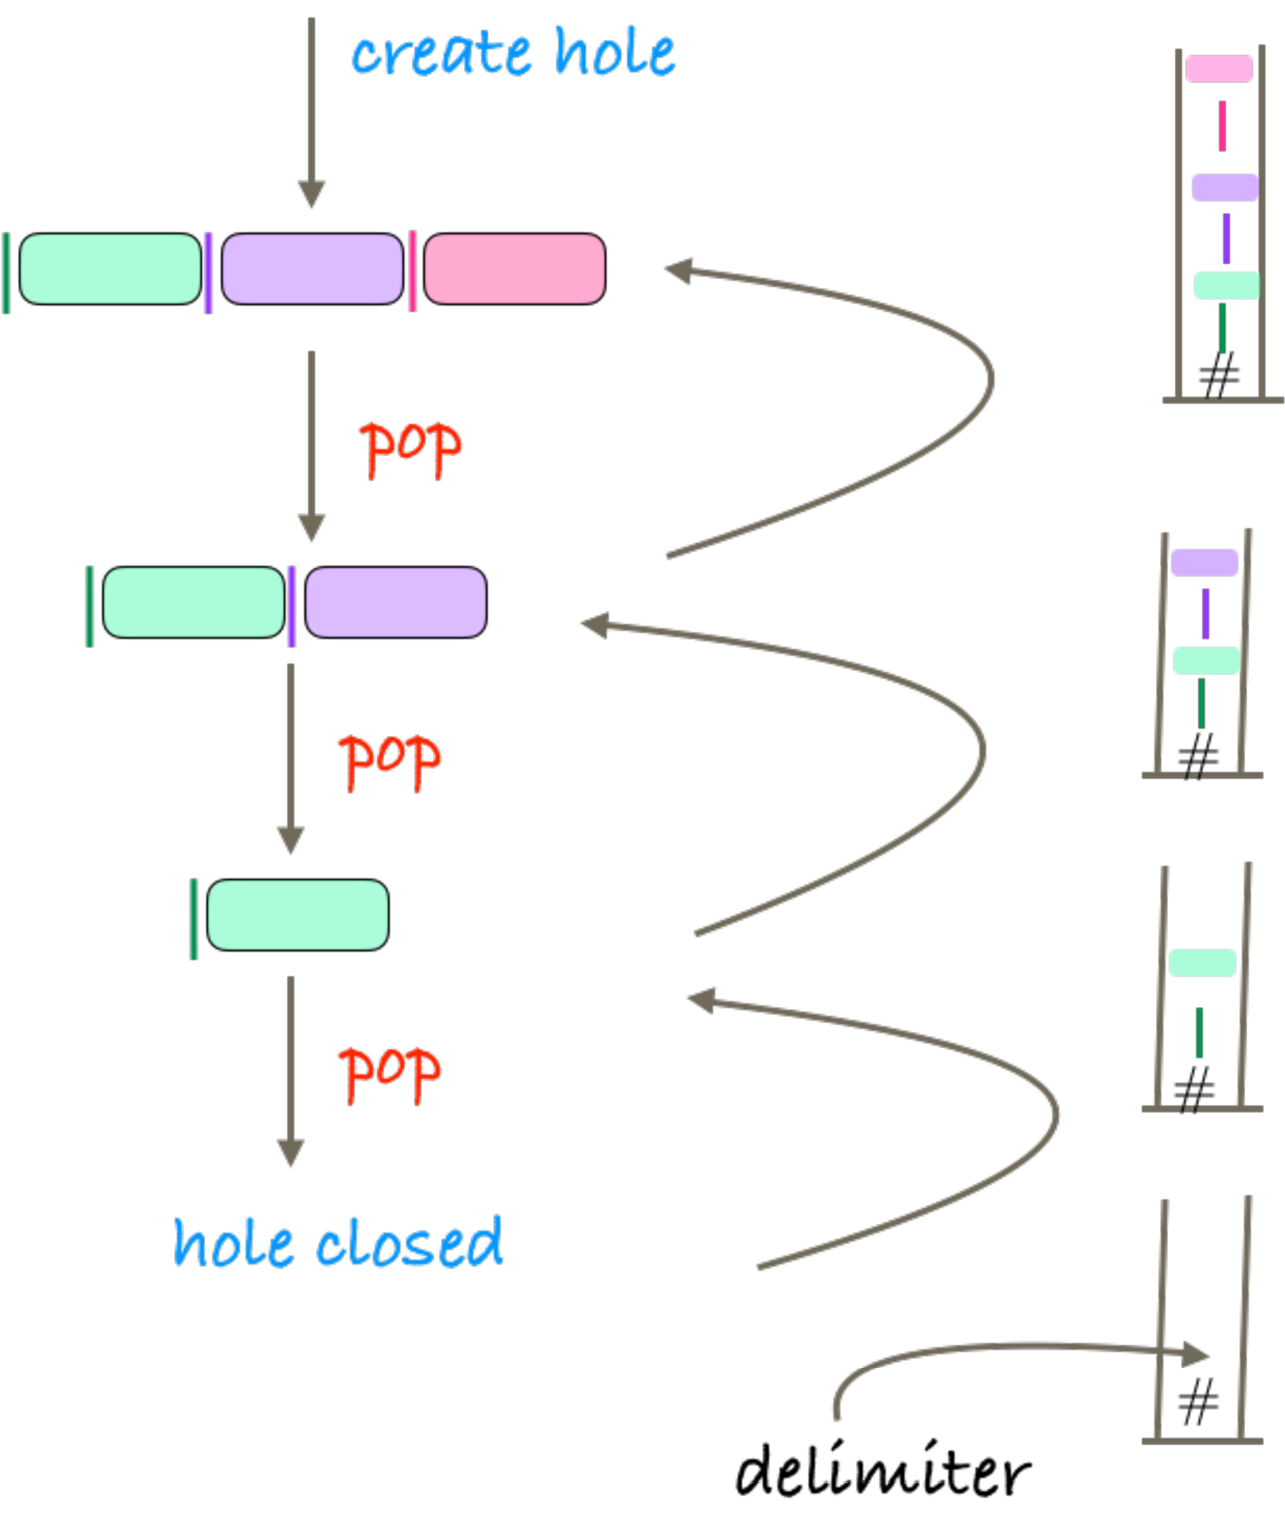
\includegraphics[scale=0.15]{fig/witness-fig.pdf}
  \end{center}
\end{frame}
%%%%%%
    \begin{frame}{Timed Automata~\mycite{alur1994theory}}
      Timed automaton is a well-studied model that capture the behaviors of
      real-time systems
      \begin{itemize}
      \item Finite States + Clocks 
     \end{itemize}
        % \begin{minipage}{0.45\textwidth}
             \begin{figure}[ht!]   
      \begin{tikzpicture}[->,thick]
        \node[initial ,initial text={}] at (0,0) (A) {
\includegraphics[scale=.1]{./fig/off.png}} ;
        \node at (3,0) (B) {
\includegraphics[scale=.1]{./fig/on.png}};
         \node at (6,0) (C) {
\includegraphics[scale=.1]{./fig/onn.png}};
        %\node[cir] at (8,.5) (D) {D};
        \path (A) edge node [below]{\scriptsize $press,\set{x}$} (B);
        \path(C) edge [bend left=30] node [above]{\scriptsize $press$}(A);
       % \path (B) edge node [above]{$3 \leq x\leq 4,\ e_2$} (D);
        \path (B)
        edge[bend right] node [above]{\scriptsize $press, x > 5$}(A);

        \path (B) edge node [above]{\scriptsize $press,x \leq 5$} (C);
      \end{tikzpicture}
     \caption{A Timed Automaton.}
    \label{fig:ex1}
  \end{figure}
 
  \begin{itemize}
     \item Infinite state space
      \item Region construction
        \item Reachability is PSPACE-C 
        \end{itemize}
      \end{frame}

%%%%%%
\begin{frame}{Extension to Time}
  We also extend the algorithm to handle Timed Multistack Pushdown
  Automata 
  \begin{itemize}
  \item  Clocks + Age (closed guards)
  \item Data Structures
    \item Timed witness generation
  \end{itemize}    
 
  \end{frame}
  %%%%%%%%%%%%%%%%%%%%
 \begin{frame}{\textcolor{blue}{BHIM}}
  \begin{itemize}
  \item We have built a tool \textcolor{blue}{BHIM\footnote{https://sparsa.github.io/bhim}} based on the algorithm
      \item Works on both timed and untimed MPDA
      \item Generates a run as a witness
        of reachability
      \item We tested our tool on a set of benchmarks
    \end{itemize}
  
    {\scriptsize \textcolor{cyan}{$^1$}https://sparsa.github.io/bhim}
    \end{frame}
  %%%%%%%%%%%%%%%%%%%
  \begin{frame}{Experiments}
      \begin{table}[t]
    \resizebox{\textwidth}{!}{ \centering
    
     \begin{tabular}{c| c| c| c| c| c| c|c } 
       \toprule
       Name & Locations & Transitions & Stacks &  Holes & Time
                                                          Empty (mili sec) &
                                                                             Time
                                                                             Witness
                                                                             (mili
                                                                             sec)
       & Memory(KB) \\ [0.5ex] 
       \hline
           
       Bluetooth & 45&89 &2 &0 &149.3&0.241
       & 6934 \\
       \hline
       

       % Bluetooth v2 &47 &134 &2 &0 &92.2 &0.176
       % & 5632\\
       % \hline
       MultiProdCons-1(2) & 11 & 18 & 2 & 2 &
                                                                               11.1&0.1

       &
         1796
        \\

       \hline
       

       MultiProdCons-2(3,2) & 7 & 11 & 2 & 2 &
                                                                                    126.529&0.281

       &
         5632
       \\
       \hline
       MultiProdCons-2(24,7) & 32 & 34 & 2 & 2 &
                                                                                      1879.33&10.63

       &
         21836
       \\
       \hline
       dm-target & 22 & 27 & 2 & 2 &
                                                              26.483&0.279

       &
         6624
       \\
       \hline
             
             

       Binary Search Tree &29 & 78 & 2 & 2 &
                                                                 60.8&5.1
       &
         5143
       \\
       \hline
       untimed-L\textsuperscript{crit} & 6 & 10 & 2 &2&14.9&0.7 &4692\\ 
       \hline
       Untimed-Maze &9 & 12 &2 &0 & 8.25&0.07 &5558\\
       \hline
    
       L\textsuperscript{bh} & 7 & 13 & 2 &2  & 22.2&0.6 &4404 \\
       
       
       \hline
      
       
       % \hyperref[sbs:dining]{Philosophers} & 11 & 13 & 2 & 2 &
       % 0.0500
       % &
       % 5244
       % \\
       
       % \hline
       % Coffee Bean & & & & & & & & \\
       \bottomrule
     \end{tabular}
   }
   % \vspace*{-1mm}
   \caption{\scriptsize Experimental results: Time Empty and Time Witness column
     represents no. of milliseconds needed for emptiness checking and
     to generate witness, respectively. }\label{tbl:experiment}
 \end{table}
    
\begin{table}[t]
  \centering \resizebox{\textwidth}{!}{
    \begin{tabular}{c| c| c| c| c| c| c| c| c| c|c}
      \toprule
      Name & Locations & Transitions & Stacks & Clocks &
                                                         c\textsubscript{max}
      &Aged(Y/N)& Holes & Time Empty(mili sec)& Time Witness (mili sec)  & Memory(KB) \\ [0.5ex] 
      \hline
           
      Bluetooth & 45 &89&2&0&2&Y&0& 152.8 & 0.119
                                                                         &5568\\
      \hline
 
      L\textsuperscript{crit}  & 6 & 10 & 2 &2&8 & Y&2 & 9965.2 &3.7 & 203396\\ 
      \hline
      Maze &9 & 12 &2 &2 &5&Y &2 &349.3&0.31&11604\\

      \hline
    
      
      \bottomrule
    \end{tabular}
  }

  \caption{\scriptsize Experimental results of timed examples. The column \cmax{}
    is defined as the maximum constant in the automaton, and Aged
    denotes if the stack is timed or not}\label{tbl:experimentTimed}
\end{table}

    \end{frame}
  %%%%%%%%%%%%% 5
   \begin{frame}{Conclusion}
   \begin{itemize}[<+->]
   \item A new underapproximation
   \item Subsumes already known underapproximations
   \item Decidable reachability
   \item BHIM
   \end{itemize}
   \end{frame}
%%%%%%%%%%%%%%%%%%%%%%%%%%%%%%%%%%%%
%   \section{Part 2: Resilience }
%   %\subsection{Motivation}
% \begin{frame}{Motivation}
%   \begin{minipage}{.3\linewidth}
%   \begin{figure}[htbp]
% \centerline{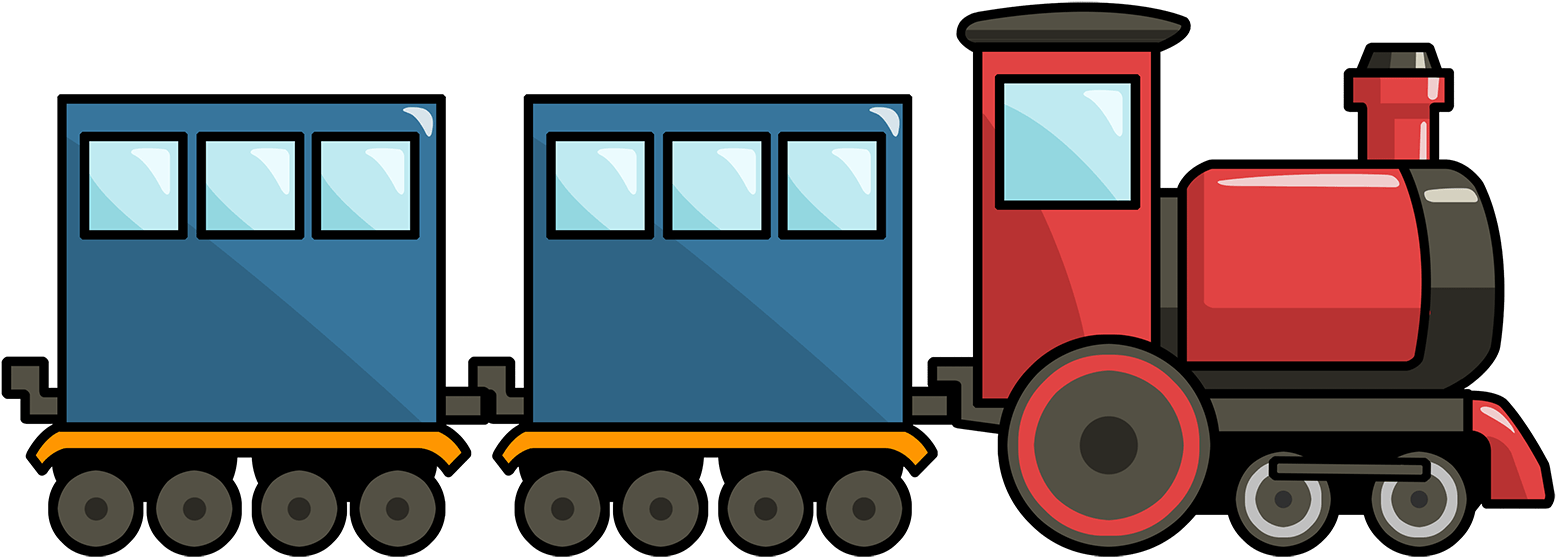
\includegraphics[width=\linewidth]{fig/rail.png}}
% \end{figure}
% \end{minipage}
% \begin{minipage}{0.6\linewidth}
%   \centerline{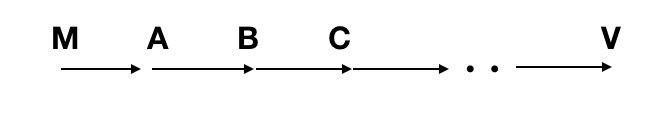
\includegraphics[width=\linewidth]{fig/stations.jpg}}
% \end{minipage}

% \begin{table}[t!]
%     \centering
%    \begin{adjustbox}{height=1.5cm}		
%     \begin{tabular}{cc}
%       \toprule
%      Stations & Time\\
%       \midrule
%      M & $T_{M}$\\
%     \midrule
%     A & $T_{A}$\\
%     \midrule
%     B & $T_{B}$\\
%     \midrule
%     C & $T_{C}$\\
%     \midrule
%     V & $T_{V}$\\
%       \bottomrule
%     \end{tabular}
%     \end{adjustbox}
%   \end{table}
  
 
%   \textbf{Question?:} If the train gets delayed in station ``B'' then,
%   can it still reach the destination ``V'' in time $T_{V}$?
% \end{frame}
% %\subsection{Modeling}
% %%%%%%%%%%%%% 5

%  \begin{frame}{Related Work}
%  \begin{itemize}
%   \item Robustness of timed autoamta~\mycite{BouyerMS11} checks the ability of the timed system to resist a slight perturbation or errors.
 
%         \item  Resilience has been considered with different meanings in
%           the following literature,
%          {\scriptsize \begin{itemize}
%             \item In \mycite{qest08} faults are modeled as conflicts,
%               the system and controller as {\em deterministic timed
%                 automata} and avoiding fault is reduced to checking
%               reachability
%               \item In~\mycite{EhlersT14} an untimed I/O automaton is
%                 considered ``sane'' if its runs contains at most $k$
%                 errors and allow a sufficient number $s$ of error-free
%                 steps in between each violation
%                 \item  Shield synthesis~\mycite{Bloem20}, that
%                   synthesizes  pre-shield (post-shield) that  shields
%                   The input (output) of a system from outside
%                   specification behaviors 
%                 \end{itemize}
%                 }
% \end{itemize}
% %            
%           \end{frame}
% %%%%%%%%%%%%
% \begin{frame}{Modeling}
%   % \begin{itemize}[<+->]
%   %   \item Timed automata is a well-known formalism to model real-time
%   %     systems
%   %     \item But, timed automata are not tailored to handle unspecified
%   %       behaviours
       
       
%   %     \end{itemize}
%       		 Our goal is to verify that the
% system \emph{recovers within boundedly many steps}, from a possibly
%  large time deviation w.r.t.  its behavior.
%  \pause 
 
% \begin{figure} [t]
%   \begin{center}
%     \scalebox{.8}{
%       \begin{tikzpicture}[->,thick]
       
%         \node[initial below,cir,initial text={}] at (5,-1) (A1)
%         {$\ell_1$} ;
%         \node[cir] at (9,-1) (B1) {$\ell_2$};
%         \node[cir1] at (1.5,-1) (C1) {$\ell_3$};
%         \node[cir1] at
%         (1.5,.3) (C3){$\ell_5$};

%         \node[cir1] at (-2,-1) (C2) {$\ell_4$};
                   
%         \path (C2) edge[bend left=15] node [midway,above,rotate=20]
%         {\scriptsize $skip$}node [midway,below]{} (C3);
%         \path (B1)
%         edge node [midway,above] {\scriptsize$arr, x\leq 4$}node
%         [midway,below]{\scriptsize$y:=0$} (A1);
%         % \path (B1)
%         % edge[-latex,bend left=40, dashed, color=red] node
%         % [midway,below]
%         % {\scriptsize$arr,4<x\leq
%         %   6$}node[above,yshift=-0.2]{\scriptsize $y:=0$} (A1);
%         \path
%         (A1) edge[bend left=50] node [midway,below]
%         {\scriptsize$x:=0$}node[above,yshift=-0.2]{\scriptsize$dep,1\leq
%           y \leq 2$} (B1);
      
%         \path (A1) edge[] node
%         [below,]{\scriptsize$late, y=0 \wedge x > 4$} (C1);
%         \path (C1)
%         edge[] node [above] {\scriptsize$dep,1 \leq y \leq 2$}
%         node[below]{\scriptsize$x:=0$} (C2);
%         \path (C3) edge[bend
%         left=15] node [above,rotate=-20]
%         {\scriptsize$arr, 6\leq x \leq 8 $}
%         node[below,rotate=-20,yshift=0.1]{\scriptsize$y:=0$} (A1);

%         \end{tikzpicture}
%       } \vspace{-\medskipamount}
%       \caption{Model $(\ta)$ of a train system with a mechanism to recover
%         from delays}
%       \label{fig:train-eg}
%     \end{center}
%     \vspace{-2\bigskipamount}
%   \end{figure}
  
% % \textcolor{red}{Question:} Given a delay in the event $arr$, can we return to its normal behavior within a finite number of steps ?
% \end{frame}

% % \begin{frame}{Example of Timed Automata}
% %     Recall that a timed automata $\ta$ is a tuple $(L,I,X,\Sigma,T,F)$
% %   and the region automata of $\ta$ is $\region{\ta}$
% %   \begin{figure}[h!]
% %     \centering
% %        %\resizebox{\textwidth}{!}{
% %         \begin{tikzpicture}[->,thick]
% %           \node[initial above,cir,initial text={}] at (-6,-1) (A)
% %           {$\ell_1$} ; \node[cir,accepting] at (-2,-1) (B) {$\ell_2$};
       
        
                
% %           \path (A) edge node [midway,above] {\scriptsize$a, 3<x< 12 \wedge y>5$}
% %           node [midway,below]{\scriptsize$y:=0$} (B); \path (B) edge[bend
% %           right=70] node [midway,below] {\scriptsize$x:=0$}node [midway,above]
% %           {\scriptsize$b,y<7$} (A);
      
% %         \end{tikzpicture}
% %      % }
% %     \end{figure}
% %   \end{frame}
%   %%%%%%%%%%%
% %\subsection{Definitions}
%       %%%%%%%%%%%%
%       \begin{frame}{Fault model and enlargement of guards}
%         \begin{itemize}[<+->]
%           \item A fault model is a map $\mathcal{P}: 
%             \Sigma \rightarrow \mathbb{Q}$.
%             \item $\faultmod(a)$ represents the possible delay of
%               action $a \in \Sigma$
%               \item A guard of a timed automata $\ta$ can be defined
%                 as,
%                 \scalebox{0.6}{$g = \underset{i\in 1..m} \bigwedge \phi_i = a_i \bowtie_{l_i} x_i
%     \bowtie_{u_i} b_i $ where
%   $a_i,b_i \in \mathbb{N}, \bowtie_{l_i}, \bowtie_{u_i} \in \{\leq, <\}$}
%   \item We define the enlargement of guards as,
%     \scalebox{0.6}{
%     $g_{\shift{\faultmod(a)}} = \!\!\!\!\underset{i\in 1..m}\bigwedge
%     \!\!\phi_i = a_i \bowtie_{l_i} x_i \leq b_i+ \faultmod(a) $ }
% \item A faulty part of the enlarged guard is,
  
% \scalebox{0.6}{
%   $g_{f,\faultmod} = \!\!\!\!\underset{i\in 1..m}\bigwedge \phi_i =$ $
%     b_i\bar \bowtie_{l_i} x_i \leq b_i+ \faultmod(a)  \mbox{ where }$ $
%   \bar \bowtie_{l_i} \in \{ <, \leq \} \setminus \bowtie_{u_i}$
% } 
%           \end{itemize}
%         \end{frame}
% %%%%%%%%%%%%%%%%%%%%%%%%%5
%         \begin{frame}{Faulty transition and faulty automata}
%           \begin{itemize}[<+->]
%             \item If there exists a fault model $\faultmod(a)$, then
%               for  transition $t = (l,g,a,R,l')$, we define a
%               faulty transition  $t_{f,\faultmod}=
%               (l,g_{f,\faultmod},a,R,\overset{\bullet}{l'}$
%               ).
%               \item For a given timed automata $\ta$ and a \emph{fault
%                 model} $\faultmod(a)$ we construct faulty automata $\faultyta$ by extending it with
%                 all possible faulty transitions.
%             \end{itemize}
%           \end{frame}
%       %%%%%%%%%%%%%%%%%%%5
%           \begin{frame}{Example}
            
%   \begin{figure} [t]
%     \begin{center}
%       \scalebox{.8}{
%         \begin{tikzpicture}[->,thick]
       
%           \node[initial below,cir,initial text={}] at (5,-1) (A1)
%           {$\ell_1$} ; \node[cir] at (9,-1) (B1) {$\ell_2$};
%           \node[cir1] at (1.5,-1) (C1) {$\ell_3$}; \node[cir1] at
%           (1.5,.3) (C3){$\ell_5$};

%           \node[cir1] at (-2,-1) (C2) {$\ell_4$};

%           \node[cir] at (5,-3) (A1f) {$\overset{\bullet}{\ell_1}$} ;
%           \node[cir] at (9,-3) (B1f)
%           {$\overset{\bullet}{\ell_2}$}; \node[cir1] at (1.5,-3) (C1f)
%           {$\overset{\bullet}{\ell_3}$}; \node[cir1] at (1.5,-1.7)
%           (C3f){$\overset{\bullet}{\ell_5}$};

%           \node[cir1] at (-2,-3) (C2f) {$\overset{\bullet}{\ell_4}$};
                   
%           \path (C2) edge[bend left=15] node [midway,above,rotate=20]
%           {\scriptsize $skip$}node [midway,below]{} (C3); \path (B1)
%           edge node [midway,above] {\scriptsize$arr, x\leq 4$}node
%           [midway,below]{\scriptsize$y:=0$} (A1); \path (B1)
%           edge[-latex, dashed, color=red] node
%           [midway,below,rotate=30]
%           {\scriptsize$arr,4<x\leq
%             6$}node[above,yshift=-0.2,rotate=30]{\scriptsize $y:=0$}
%           (A1f); \path (A1) edge[bend left=50] node [midway,below]
%           {\scriptsize$x:=0$}node[above,yshift=-0.2]{\scriptsize$dep,1\leq
%             y \leq 2$} (B1);
      
%           \path (A1) edge[] node
%           [below,]{\scriptsize$late, y=0 \wedge x > 4$} (C1); \path
%           (C1) edge[] node [above] {\scriptsize$dep,1 \leq y \leq 2$}
%           node[below]{\scriptsize$x:=0$} (C2); \path (C3) edge[bend
%           left=15] node [above,rotate=-20]
%           {\scriptsize$arr, 6\leq x \leq 8 $}
%           node[below,rotate=-20,yshift=0.1]{\scriptsize$y:=0$} (A1);

         
%           \path (C2f) edge[bend left=15] node [midway,above,rotate=20]
%           {\scriptsize $skip$}node [midway,below]{} (C3f); \path (B1f)
%           edge node [near start,above] {\scriptsize$arr, x\leq 4$}node
%           [near start,below]{\scriptsize$y:=0$} (A1f);
         
%           \path (A1f) edge[bend right=50] node [midway,below]
%           {\scriptsize$x:=0$}node[above,yshift=-0.2]{\scriptsize$dep,1\leq
%             y \leq 2$} (B1f);
      
%           \path (A1f) edge[] node
%           [below,]{\scriptsize$late, y=0 \wedge x > 4$} (C1f); \path
%           (C1f) edge[] node [above] {\scriptsize$dep,1 \leq y \leq 2$}
%           node[below]{\scriptsize$x:=0$} (C2f); \path (C3f) edge[bend
%           left=15] node [above,rotate=-20]
%           {\scriptsize$arr, 6\leq x \leq 8 $}
%           node[below,rotate=-20,yshift=0.1]{\scriptsize$y:=0$} (A1f);
         
%         \end{tikzpicture}
%       } \vspace{-\medskipamount}
%       \caption{Enlarged automaton $\ta_{\faultmod}$ for the train
%         system $\ta$ and fault model $\faultmod(arr)=2$ (with recovery)
%         model of Figure~\ref{fig:train-eg}}
%       \label{fig:train-eg-faulty}
%     \end{center}
%     \vspace{-2\bigskipamount}
%   \end{figure}
	
%     %       \begin{figure} [t]
%   %     \begin{center}
%   %     \resizebox{\textwidth}{!}{
%   %       \begin{tikzpicture}[->,thick]
%   %         \node[initial above,cir,initial text={}] at (-6,-1) (A)
%   %         {$\ell_1$} ; \node[cir,accepting] at (-2,-1) (B) {$\ell_2$};
       
%   %         \node[initial above,cir,initial text={}] at (5,-1) (A1)
%   %         {$\ell_1$} ; \node[cir,accepting] at (9,-1) (B1) {$\ell_2$};
%   %         \node[cir1,accepting] at (0,-1) (C1)
%   %         {$\overset{\bullet}{\ell_2}$};

%   %         \node[cir1] at (4,1.1) (C2) {$\overset{\bullet}{\ell_1}$};
                
%   %         \path (A) edge node [midway,above] {\scriptsize$a, 3<x< 12 \wedge y>5$}
%   %         node [midway,below]{\scriptsize$y:=0$} (B); \path (B) edge[bend
%   %         right=70] node [midway,below] {\scriptsize$x:=0$}node [midway,above]
%   %         {\scriptsize$b,y<7$} (A);
       
        
%   %         \path (A1) edge node [midway,above]
%   %         {\scriptsize$a, 3<x< 12 \wedge y>5$}node [midway,below]{\scriptsize$y:=0$} (B1);
%   %         \path (B1) edge[bend right=50] node [midway,below]
%   %         {\scriptsize$x:=0$}node[above,yshift=-0.2]{\scriptsize$b,y<7$} (A1);
       
      
%   %         \path (A1) edge node [left,below]
%   %         {\scriptsize$y:=0$}node
%   %         [right,above]{\scriptsize$a, 12 \leq x \leq 14 \wedge y>5$} (C1); \path (C1) edge[bend left=40]
%   %         node [above,rotate=35] {\scriptsize$b,y<7$}
%   %         node[below,rotate=35]{\scriptsize$x:=0$} (C2); \path (C2) edge[bend
%   %         left=5] node [above,rotate=29] {\scriptsize$a, 3<x< 12 \wedge y>5$}
%   %         node[below,rotate=29,yshift=0.1]{\scriptsize$y:=0$} (C1); \path (B1) edge[bend
%   %         right=40] node [below,rotate=-23]
%   %         {\scriptsize$x:=0$}node[above,rotate=-23]{\scriptsize$b,y= 7$} (C2);
%   %       \end{tikzpicture}
%   %     }
%   %     \caption{\scriptsize{$\ta$ on the left; Enlargement $\ta_{\faultmod}$ on the
%   %       right, $\faultmod(a)=2, \faultmod(b)=0$.}}
%   %     \label{faulty-eg}
%   %   \end{center}
		
%   % \end{figure}
%         \end{frame}
%         %%%%%%%%%%%%%%%%%% 5
       
%           %%%%%%%%%%%%%%%%%%%%%%%5
%         \begin{frame}{Back to Normal and Resilience}
%           \begin{block}{Just faulty run of $\faultyta$}
%             A just faulty run is a minimal prefix of a run of $\faultyta$ that ends with a fault
%             \end{block}
%           \begin{block}{Back to Normal (BTN)}
%           For a just faulty run $\rho_{P}$, is it possible for
%             $\faultyta$ to extend $\rho_{P}$ such that it can mimic a non-faulty run of $\ta$ after $K$
%             steps of the fault?
%           \end{block}
%           \pause
%             \begin{enumerate}[<+->]
%             \item Always? (All extension of the faulty run)
%             \item Some? (At-least one extension of the faulty run)
%             \end{enumerate}
            
%             \pause
            
%             {\vspace{-1.3cm} \hspace{7cm} \textcolor{red}{$\forall\mbox{-}resilience$!}}
%            % \pause
% %            \vspace{1.5cm}
% %            {\hspace{-1cm}\textcolor{red}{$\exists\mbox{-}resilience$!}}
            
%             \pause
           
%             \hspace{8.3cm}\vspace{5cm}
%             \textcolor{red}{$\exists\mbox{-}resilience$!}
            
%             \pause
%             When we consider \textcolor{blue}{untimed} runs, we call it \textcolor{blue}{untimed BTN} and
%             \textcolor{blue}{untimed Resilience} respectively.
%         \end{frame}
%         %%%%%%%%%%%%%%%%

%         \begin{frame}{Example Revisited}
          
%   \begin{figure} [t]
%     \begin{center}
%       \scalebox{.6}{
%         \begin{tikzpicture}[->,thick]
       
%           \node[initial below,cir,initial text={}] at (5,-1) (A1)
%           {$\ell_1$} ; \node[cir,accepting] at (9,-1) (B1) {$\ell_2$};
%           \node[cir1] at (1.5,-1) (C1) {$\ell_3$}; \node[cir1] at
%           (1.5,.3) (C3){$\ell_5$};

%           \node[cir1] at (-2,-1) (C2) {$\ell_4$};

%           \node[cir] at (5,-3) (A1f) {$\overset{\bullet}{\ell_1}$} ;
%           \node[cir,accepting] at (9,-3) (B1f)
%           {$\overset{\bullet}{\ell_2}$}; \node[cir1] at (1.5,-3) (C1f)
%           {$\overset{\bullet}{\ell_3}$}; \node[cir1] at (1.5,-1.7)
%           (C3f){$\overset{\bullet}{\ell_5}$};

%           \node[cir1] at (-2,-3) (C2f) {$\overset{\bullet}{\ell_4}$};
                   
%           \path (C2) edge[bend left=15] node [midway,above,rotate=20]
%           {\scriptsize $skip$}node [midway,below]{} (C3); \path (B1)
%           edge node [midway,above] {\scriptsize$arr, x\leq 4$}node
%           [midway,below]{\scriptsize$y:=0$} (A1); \path (B1)
%           edge[-latex, dashed, color=red] node
%           [midway,below,rotate=30]
%           {\scriptsize$arr,4<x\leq
%             6$}node[above,yshift=-0.2,rotate=30]{\scriptsize $y:=0$}
%           (A1f); \path (A1) edge[bend left=50] node [midway,below]
%           {\scriptsize$x:=0$}node[above,yshift=-0.2]{\scriptsize$dep,1\leq
%             y \leq 2$} (B1);
      
%           \path (A1) edge[] node
%           [below,]{\scriptsize$late, y=0 \wedge x > 4$} (C1); \path
%           (C1) edge[] node [above] {\scriptsize$dep,1 \leq y \leq 2$}
%           node[below]{\scriptsize$x:=0$} (C2); \path (C3) edge[bend
%           left=15] node [above,rotate=-20]
%           {\scriptsize$arr, 6\leq x \leq 8 $}
%           node[below,rotate=-20,yshift=0.1]{\scriptsize$y:=0$} (A1);

         
%           \path (C2f) edge[bend left=15] node [midway,above,rotate=20]
%           {\scriptsize $skip$}node [midway,below]{} (C3f); \path (B1f)
%           edge node [near start,above] {\scriptsize$arr, x\leq 4$}node
%           [near start,below]{\scriptsize$y:=0$} (A1f);
         
%           \path (A1f) edge[bend right=50] node [midway,below]
%           {\scriptsize$x:=0$}node[above,yshift=-0.2]{\scriptsize$dep,1\leq
%             y \leq 2$} (B1f);
      
%           \path (A1f) edge[] node
%           [below,]{\scriptsize$late, y=0 \wedge x > 4$} (C1f); \path
%           (C1f) edge[] node [above] {\scriptsize$dep,1 \leq y \leq 2$}
%           node[below]{\scriptsize$x:=0$} (C2f); \path (C3f) edge[bend
%           left=15] node [above,rotate=-20]
%           {\scriptsize$arr, 6\leq x \leq 8 $}
%           node[below,rotate=-20,yshift=0.1]{\scriptsize$y:=0$} (A1f);
         
%         \end{tikzpicture}
%       } 
%       \label{fig:train-eg-faulty}
%     \end{center}
    
%   \end{figure}
	
               
%   %         \begin{figure} [t]
%   %     \begin{center}
%   %     \resizebox{\textwidth}{!}{
%   %       \begin{tikzpicture}[->,thick]
%   %         \node[initial above,cir,initial text={}] at (-6,-1) (A)
%   %         {$\ell_1$} ; \node[cir,accepting] at (-2,-1) (B) {$\ell_2$};
       
%   %         \node[initial above,cir,initial text={}] at (5,-1) (A1)
%   %         {$\ell_1$} ; \node[cir,accepting] at (9,-1) (B1) {$\ell_2$};
%   %         \node[cir1,accepting] at (0,-1) (C1)
%   %         {$\overset{\bullet}{\ell_2}$};

%   %         \node[cir1] at (4,1.1) (C2) {$\overset{\bullet}{\ell_1}$};
                
%   %         \path (A) edge node [midway,above] {\scriptsize$a, 3<x< 12 \wedge y>5$}
%   %         node [midway,below]{\scriptsize$y:=0$} (B); \path (B) edge[bend
%   %         right=70] node [midway,below] {\scriptsize$x:=0$}node [midway,above]
%   %         {\scriptsize$b,y<7$} (A);
       
        
%   %         \path (A1) edge node [midway,above]
%   %         {\scriptsize$a, 3<x< 12 \wedge y>5$}node [midway,below]{\scriptsize$y:=0$} (B1);
%   %         \path (B1) edge[bend right=50] node [midway,below]
%   %         {\scriptsize$x:=0$}node[above,yshift=-0.2]{\scriptsize$b,y<7$} (A1);
       
      
%   %         \path (A1) edge node [left,below]
%   %         {\scriptsize$y:=0$}node
%   %         [right,above]{\scriptsize$a, 12 \leq x \leq 14 \wedge y>5$} (C1); \path (C1) edge[bend left=40]
%   %         node [above,rotate=35] {\scriptsize$b,y<7$}
%   %         node[below,rotate=35]{\scriptsize$x:=0$} (C2); \path (C2) edge[bend
%   %         left=5] node [above,rotate=29] {\scriptsize$a, 3<x< 12 \wedge y>5$}
%   %         node[below,rotate=29,yshift=0.1]{\scriptsize$y:=0$} (C1); \path (B1) edge[bend
%   %         right=40] node [below,rotate=-23]
%   %         {\scriptsize$x:=0$}node[above,rotate=-23]{\scriptsize$b,y= 7$} (C2);
%   %       \end{tikzpicture}
%   %     }
%   %     \caption{\scriptsize{$\ta$ on the left; Enlargement $\ta_{\faultmod}$ on the
%   %       right, $\faultmod(a)=2, \faultmod(b)=0$.}}
%   %     \label{faulty-eg}
%   %   \end{center}
		
%   % \end{figure}
%   \pause
%     {\scriptsize The run
%     $\rho_f=(\ell_{1},0|0)\overset{(t_{12},2)}{\longrightarrow}(\ell_{2},0|2)\overset{(\overset{\bullet}{t_{21}},8)}{\longrightarrow}(\ell_{1},6|0)\overset{(t_{13},8)}{\longrightarrow}(\overset{\bullet}{\ell_{3}},6|0)\overset{(t_{34},10)}{\longrightarrow}(\overset{\bullet}{\ell_{4}},0|2)\overset{(t_{45},10)}{\longrightarrow}(\overset{\bullet}{\ell_5},0|2)\overset{(t_{51},18)}{\longrightarrow}(\overset{\bullet}{\ell_{1}},8|0)\overset{(t_{12},19)}{\longrightarrow}(\overset{\bullet}{\ell_{2}},0|1)$ of $\ta_{\faultmod}$
%     reading  the word $(dep,2)\textcolor{red}{(arr,8)(late,8)(dep,10)(skip,10)}\textcolor{green}{(arr,18)(dep,19)}$
%      % reading word $w_{\rho}=(a,14)(b,20)(a,31)$
%     is 4-BTN
    
%     because of the run
%   $\rho=(\ell_{1},0|0)\overset{(t_{12},2)}{\longrightarrow}(\ell_{2},0|2)\overset{(t_{21},6)}{\longrightarrow}(\ell_{1},4|0)\overset{(t_{12},8)}{\longrightarrow}(\ell_{2},0|2)\overset{(t_{21},12)}{\longrightarrow}(\ell_{1},4|0)\overset{(t_{12},14)}{\longrightarrow}(\ell_{2},0|2)\overset{(t_{21},18)}{\longrightarrow}(\ell_{1},4|0)\overset{(t_{12},19)}{\longrightarrow}(\ell_{2},0|1)$
%   of $\ta$
%     reading the word $(dep,2)(arr,6)(dep,8)(arr,12)(dep,14)\textcolor{green}{(arr,18)(dep,19)}$. }
% \end{frame}
% %%%%%%%%%%%%%%%%%%%%%%%%%%%%5
%        % \subsection{Contributions}
% \begin{frame}{Results}
%   \begin{table}[t!]
%     \centering
%     \resizebox{.7\linewidth}{!}{
%           \begin{tabular}{lll}
%       \toprule
%       \rowcolor{Gray}		
%                  &  Universal Resilience & Existential Resilience \\
%       \midrule
%       Timed         & Undecidable for TA  &  EXPSPACE  \\
%                        &  EXPSPACE-C for IRTA  & PSPACE-Hard   \\
%       \hline
			
      
                                                            
      
%       Untimed                 & EXPSPACE-C  & PSPACE-C    \\  
     

%       \bottomrule

% \end{tabular}
% }
% \caption{Summary of results for resilience. 
% %For all results, Existential resilience has better complexity/decidability than
%   %universal resilience, by at least an exponential factor.
% 	}
% \label{tab:results-timed}
% %\vspace{-2\bigskipamount}
% \end{table}
% \end{frame}
% %\subsection{Untimed Resilience}
% %%%%%%%%%%%%%%% 5

% \section{Part 3: Randomness}
%   %\subsection{Motivation}
%   \begin{frame}{Motivation}
%     \begin{figure}
%       \begin{center}

%       \begin{tikzpicture}[->,thick]
%         \node[initial, dia, initial text ={}] at (0,0) (A) {J} ;
%         \node[dia] at (6,0) (B) {F};
%       \node[cir] at (2,0) (C) {S};
      
%        \node[dia] at (4,0) (C1) {C};
    
%        \path (A) edge node[ above] {New Job} (C);
%        \path (C) edge [bend left] node[above] {Schedule} (C1);
%        \path(C1) edge [bend left] node [below] {Interrupt} (C);
%        \path(C1) edge node [above] {Finished} (B);
     
       
%       \end{tikzpicture}
  
  
%      % \caption{An example of }
%     \label{fig:ex1}
%   \end{center}
% \end{figure}
% \begin{itemize}
% \item A scheduler ``S'' schedules new 
%   jobs to the CPU ``C''
%   \item The scheduler is stochastic
% \item Every job has a CPU time requirement T  to complete
   
% \end{itemize}
% Is it possible to finish a newly added job within
%     some total time T\textsubscript{f}.
% \end{frame}
% %%%%%%%%%%%%%%%%%%%%%%5
%   %\subsection{Modeling }
  
%       %%%%%%%%%%%%%%%%%%%
   
%      \begin{frame}{Time + Probability}
%        \begin{itemize}
%          \item Randomized delays and discrete
%            choices~\mycite{Baier2008,Baier2007}
%            \item Purely stochastic models might not be sufficient in
%              real world problems
%              \item Interactions with the environment
%          \end{itemize}
%       \end{frame}
%       %%%%%%%%%%%%%%%%%
      
%       \begin{frame}{Stochastic Timed Games (STG) \mycite{icalp09}}
%         \begin{itemize}
%         \item Locations partitioned to players with competing
%           objectives
%           \begin{itemize}
%           \item Some locations belong to the environment and  are
%             probabilistic ($\ocircle$).
%             \item Others belong to either player $\square$  or
%               $\Diamond$.
%               \item The environment is the \half-player.
%             \end{itemize}
%         \item \twohalf-player,
%           \begin{itemize}
%             \item $\square + \Diamond + \ocircle$ 
%           \end{itemize}
%         \item \onehalf-player,
%           \begin{itemize}
%             \item $\Diamond + \ocircle$ 
%           \end{itemize}
%         \item \half-player -- just the environment ($\ocircle$)
          
%         \end{itemize}
       
%       \end{frame}
%       %%%%%%%%%%%%%
      
%       \begin{frame}{Qualitative reachability vs. Quantitative reachability}
%         \begin{alertblock}{Reachability Question}
%           \scriptsize
%           Given a \twohalf-STG (resp. \onehalf-STG) \stg{} with a set T of target locations, an
%           initial state $s_0$, and a threshold $ p$ does
%           there exists a strategy of player $\Diamond$ ( resp. $\square$)
%           such that for every strategy of other players, the 
%           player $\Diamond$ (resp. $\square$)  can reach target T from $s_0$
%           with probability $\bowtie p$?
%           \pause
%           \end{alertblock}
%         \begin{block}{Qualitative reachability:}
%          The constraint on probability $ p\in \set{0, 1}$
%         \end{block}
%         \begin{block}{Quantitative reachability:}
%            The constraint on probability $ 0 < p < 1$
           
%         \end{block}
        
%       \end{frame}

%       %%%%%%%%%%%%%%%%%% 5
%     %  \subsection{Known Results}
%       \begin{frame}{Known results on STG}
       
%         \begin{table}[]
%            \resizebox{\textwidth}{!}{
%           \begin{tabular}{cccc}
%             Model                & \#-Clocks & Qualitative                   & Quantitative                                                               \\
%             \hline
% \multirow{2}{*}{\half-Player}    & 1         & Decidable~\mycite{Baier2008}  & Decidable~\mycite{Jurdzinski2008}                                            \\
%                                  & n         & {\bf Open}                    & {\bf Open}                                                                 \\
%             \hline
% \multirow{2}{*}{\onehalf-Player} & 1         & Decidable~\mycite{icalp09}
%                                  & Decidable (initialized\footnote{})~\mycite{Akshay2016}                                                                 \\
%                                  & n         & {\bf Open}                    & Undecidable~\mycite{Akshay2016}
%                                                                                                                                                           \\
%             \hline
% \multirow{2}{*}{\twohalf-Player} & 1         & Decidable~\mycite{Akshay2016} & Decidable (initialized\footnotemark[\value{footnote}]~\mycite{Akshay2016}) \\
%                                  & n         & {\bf Open}                    & Undecidable~\mycite{icalp09}                                               \\
%             \hline
%           \end{tabular}}
        
% \end{table}
% {\scriptsize \textcolor{cyan}{$^2$}Initialized: Any transition from non-stochastic to stochastic
%   location resets the clock}
%         \end{frame} 
%         %%%%%%%%%%%%%%%%%
%        % \subsection{Definitions}
%         \begin{frame}{StopWatches}
%      \begin{block}{StopWatches} Clocks with derivative zero at some locations
%      \end{block}
%      \begin{itemize}[<+->]
%        \item Can simulate linear hybrid automata~\mycite{Cassez2000}
%      \item Reachability is \textcolor{red}{Undecidable!}
%      \item Useful in job-scheduling~\mycite{Abdeddaim2002}
       
%      \end{itemize}

%      \end{frame}
%      %%%%%%%%%%%%%%%%%%%% 5
     
%      \begin{frame}{Stochastic StopWatch Games (SSG)}
%        \begin{itemize}
%        \item Extension of  STG
%          \item Clocks are replaced with StopWatches
%          \end{itemize}
%                \begin{figure}[ht!]
%   \begin{center}
%     \begin{figure}
%       \begin{center}

%       \begin{tikzpicture}[->,thick]
%         \node[initial, dia, initial text ={}] at (0,0) (A) {J} ;
%         \node[dia, accepting] at (9,0) (B) {F};
%       \node[cir1] at (3,0) (C) {S};
      
%        \node[dia] at (6,0) (C1) {C};
    
%        \path (A) edge node[ above] {New Job} node[below] {$\set{x,x_c}$} (C);
%        \path (C) edge [bend left] node[above] {Schedule} (C1);
%        \path(C1) edge [bend left] node [below] {Interrupt} (C);
%        \path(C1) edge node [above] {Finished} node [below] {$x_c == T
%          \wedge x \leq T_f$}
%           (B);
     
       
%       \end{tikzpicture}
  
  
%      % \caption{An example of }
%     \label{fig:ex1}
%   \end{center}
% \end{figure}
  
  
    
%     \label{fig:ex1}
%   \end{center}
% \end{figure}
% \begin{itemize}
%   \item The stochastic scheduler  can be modeled as a
%     $1\frac{1}{2}$ SSG with a clock $x$ and a stopwatch $x_c$
%   \item The stopwatch only measures time when it is in CPU ``C''
   
%   \end{itemize}
%         \end{frame}
%         %%%%%%%%%%%%%%%
%       % \subsection{Contributions}
%        \begin{frame}{Results}
%          \begin{block}{Results}
%            For $\onehalf$-Player SSG Qualitative reachability,
%            \begin{itemize}
% \item         is decidable with 2 stopwatches and is EXPTIME-C
% \item    is undecidable with 3 stopwatches.
%   \end{itemize}
%          \end{block}
% %           \begin{table}[]
% %            \resizebox{\textwidth}{!}{
% %           \begin{tabular}{ccc}
% %             Model& \#-StopWatches & Qualitative Reachability    \\
% %             \hline
% % \multirow{2}{*}{\onehalf-Player-SSG} &2 &Decidable (EXPTIME-Complete)\\
                                                
% %                  & 3  & Undecidable  \\
% %             \hline
% %           \end{tabular}}
        
% % \end{table}
        
%           \end{frame}
%           %%%%%%%%%%%%%%%%%
         
%           \begin{frame}{EXPTIME-Completeness I}
%             \begin{block}{Region graph}
%               One can construct a region graph
%               of a stopwatch automata with two stopwatches
%               \end{block}
%              Membership:
%             \begin{itemize}
%             \item Backward fixed point algorithm on region graph of
%               the \onehalf-player SSG with 2 stopwatches.
%               \item The region graph is exponential to the model
%               \item Algorithm is polynomial in the size of the graph
%               \end{itemize}
%             \end{frame}
%             %%%%%%%%%%%%% 5
%             \begin{frame}{EXPTIME-Completeness II}
%               Hardness:
%               \begin{itemize}
%                 \item Qualitative reachability problem of
%                   probabilistic timed automata (PTA) with two clocks is
%                   EXPTIME-Complete~\mycite{Kwiatkowska2000}
%                     \item We can build a \onehalf-SSG \stg with two
%                       stopwatches corresponding a two clock PTA $\mathcal{P}$
%                      \item By solving qualitative reachability of \stg
%                        one can solve qualitative reachability of $\mathcal{P}$.
%                      \end{itemize}
%                    \end{frame}
%                     %%%%%%%%%%%%%%%%%
           
%             \begin{frame}{Two Counter Machine}
%               \begin{block}{Two Counter Machine} \scriptsize
%                 A two counter machine $\mathcal{M}$ can be defined as a tuple $(L,\mathcal{C})$, where $L$ is the
% finite state of instructions including the special instruction
% ``HALT'', and $\mathcal{C}=\{C_{1},C_{2}\}$. The instruction can be any one of the
% following types,
%  \end{block}
% \begin{itemize}\scriptsize
% \item  (Increment the counter) $\ell_{p}$ : $C_{i}$ := $C_{i}+1; \textrm{ goto } \ell_{q};$,
% \item  (Decrement the counter)
%   $\ell_{p}$: $C_{i}$:= $C_{i}-1; \textrm{ goto } \ell_{q};$,
%   \item (Checking zero)
%   $\ell_{p}$: $\textrm{ if}~(C_{i} = 0) \textrm{ then goto } \ell_{q}$
%   else goto $\ell_{r};$,
%   \item (Halting instruction) $\ell_{q}$ : HALT;
%   \end{itemize}
% \end{frame}
% %%%%%%%%%%%%%%%%%%%%%5
%   \begin{frame}{Undecidability}
%   \begin{block}{Non halting problem of 2-counter machine~\mycite{10.5555/1095587}}\scriptsize
%    The non halting problem for
% two-counter machine is undecidable
%     \end{block}
%               \begin{alertblock}{Theorem}\scriptsize Given a two counter machine $\mathcal{M}$, one can build
%               a \onehalf-player SSG with three stopwatches, such that,
%               the player will have a strategy to reach the target
%               location T, if and only if the two counter machine does
%               not halt.
%             \end{alertblock}
%             \pause
%              \begin{exampleblock}{\scriptsize Qualitative Reachability of
%                 \onehalf-player SSG with three stopwatches is Undecidable}
%               \end{exampleblock}
%             \end{frame}
                  
%             %%%%%%%%%%%%%%%
%             \begin{frame}{Gadget for Decrementing Counter $C_1$}
%                 \begin{figure} [!ht]
%     \begin{center}
%       \resizebox{\textwidth}{!}{
%         \begin{tikzpicture}[->,thick]
%           \tikzstyle{cir}=[draw, circle,minimum size=1.4em,inner
%           sep=0em] \tikzstyle{dia}=[draw,diamond,minimum
%           size=1.4em,inner sep=0em]
                                                                                                                                                                         
%           \node[initial, dia, initial text
%           ={$x=\frac{1}{2^i3^j},y=0,z=0$}] at (-10,-6) (A) {$\ell_i$}
%           ;
    
%           \node[dia] at (-8,-6) (B) {$B$};
%           \node[dia,fill=blue!50] at
%           (-6,-6) (C) {$C$}; \node[dia] at (-4,-6) (D) {$D$};
%           \node[cir] at (-2,-6) (A6) {$E$};
%           \node[dia] at (-1,-8) (L)
%           {$\ell_j$};
%           \node[draw=blue, fill=red!20, rectangle,
%           accepting] at (-3,-8) (T) {$T$};

%           \path (A) edge node
%           [above]{$x=1?$} (B);
%           \path (A) edge node [below]{$\{x,y\}$} 
%           (B);
%           \path (B) edge node [above]{$z=1?$} node
%           [below]{$\{z\}$} (C);
%           \path (C) edge node [above]{$y=1?$}
%           node[below]{$\{y\}$} (D);
%           \path (D) edge node
%           [above]{$z=1?$} node[below]{$\{z,y\}$} (A6);
%           \path (A6) edge
%           node [right]{$z=0?$} (L);
%           \path (A6) edge node
%           [left]{$z=0?$} (T);
%         \end{tikzpicture}
%       }
      
%       \caption{Gadget Dec $C_1$}
%       \label{fig:dec-c1-3var}
%     \end{center}
%   \end{figure}
%   \begin{itemize}
%     \item  On entry to node
%       $\ell_i$, we have the values $x=\frac{1}{2^i3^j}$, $y=z=0$
%     \item On node $C$  rate of $x = 0$
%       \item At the stochastic node $E$
%     the valuation
%     $x=\frac{2}{2^{i}3^j} =
%     \frac{1}{2^{i-1}3^{j}}$,$y=z=0$
%     \item From the
%     stochastic node $E$, $\ell_j$ and $T$ can be reached with
%     probability $=\frac{1}{2}$ each
%     \end{itemize}
%   \end{frame}
%   %%%%%%%%%%%%%%%%%%%%%%%%%%%
%   \begin{frame}{Simulating Two counter Machine}
%     \begin{block}{Theorem}
%   Given a two counter machine $\cal{M}$, Player $\Diamond$ has a
%   strategy to reach a target node $T$  with probability 1
%   in the constructed game graph $G(\cal{M})$ \Iff the two counter
%   machine $\cal{M}$ does not halt.
% \end{block}
% \begin{itemize}
%   \item Every gadget reaches the next location $\ell_j$ and target
%     location $T$ with probability $\half$ each.
%     \item Probability of reaching a target T in $G(\cal{M})$ is $P_{total} = \half
%       + \half\times P_{rest}$
%       \item If M reaches HALT, then we reach a T with probability < 1
        
%         \item If it M doesn't reach HALT, then it will run infinitely
%           and $P_{total} = \sum_{n=1}^\infty 2^{-n} = 1$
%   \end{itemize}
%     \end{frame}
         
%     %%%%%%%%%%%%%%%%%%%%%%%%%%%
%     \section{Conclusion}
%     \begin{frame}{Conclusion}
%       \begin{itemize}
%         \item In this thesis, we try to solve the following problems 
%           \begin{enumerate}[<+->]
%           \item Modeling multi-threaded \textcolor{red}{R}ecursive systems such that it is more expressive with decidable reachability and its extension to the timed system
%           \item Methodology of checking \textcolor{red}{R}esilience of timed systems modeled in timed automata
%           \item Modeling \textcolor{red}{R}andomness in timed systems using stochastic timed games.
          
%             \end{enumerate}
%         \end{itemize}
%     \end{frame}
%     %%%%%%%5
%     \begin{frame}{Conclusion Contd.}
%     \begin{enumerate}
%         \item The 3\textcolor{red}{R}s combined increases the boundary of what timed automata can model.
%     \item We also studied what can be the limitation of timed automata in modeling 3\textcolor{red}{R}s
%     \item As a result of this work, we have a tool solving \textcolor{red}{R}ecursion,
%     \item a methodology to capture faulty timed automata,
%     \item and a new model to capture \textcolor{red}{R}andomness in timed systems
%     \end{enumerate}
%     \end{frame}
%     %%%%%%%%%%%%%%%%%%%%%%%%
%             \section{Future work}
%             \begin{frame}{Future work}
%               \begin{itemize}
%               \item Recursion:
%                 \begin{itemize}
%                 \item Symbolic representation and open guards
%                   \item Dynamic stack addition and removal
%                   \end{itemize}
%                 \item Resilience:
%                   \begin{itemize}
%                     \item Continuous resilience
%                     \end{itemize}
%                   \item Randomness:
%                     \begin{itemize}
%                       \item \twohalf-Player SSG under bounded time
%                         constraint
%                         \end{itemize}
%                 \end{itemize}
%             \end{frame}
%             %%%%%%%%%%%%%%%%%%%%%%%%
%             \begin{frame}{List of Publications}
%               \begin{enumerate}
%                 \item S. Akshay, Paul Gastin, Krishna S, \emph{Sparsa
%                   Roychowdhury} \textbf{Revisiting Underapproximate
%                   Reachability for Multipushdown Systems} \textcolor{blue}{TACAS'20}
%                   \item S. Akshay, Blaise Genest, Loic Helouet,
%                     Krishna S and \emph{Sparsa Roychowdhury} \textbf{Resilience of
%                     Timed Systems} \textcolor{blue}{FSTTCS'21}
%                     \item \emph{Sparsa Roychowdhury} \textbf{\onehalf-Player Stochastic StopWatch Games} \textcolor{blue}{TIME'21 }
%                   \end{enumerate}
%               \end{frame}
              
 \begin{frame}{Thank You}
   \begin{center}
     \Huge{Thank You}\\
     \end{center}
     \end{frame}
%      \begin{frame}{Thank You}
% \centering
% 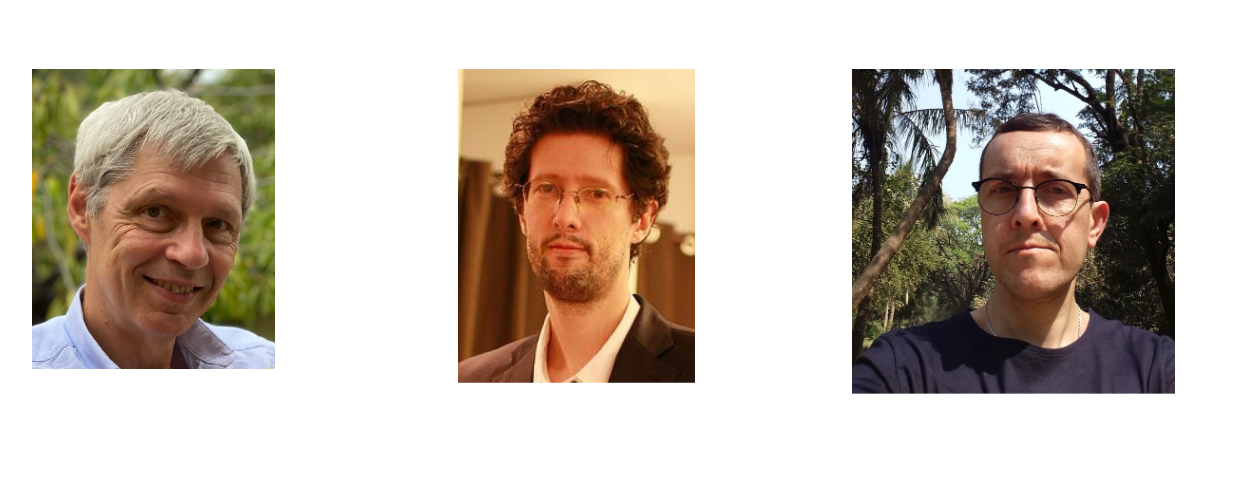
\includegraphics[width=\textwidth]{fig/image.png}
% \end{frame}
% \begin{frame}{Thank You}
% \centering
% 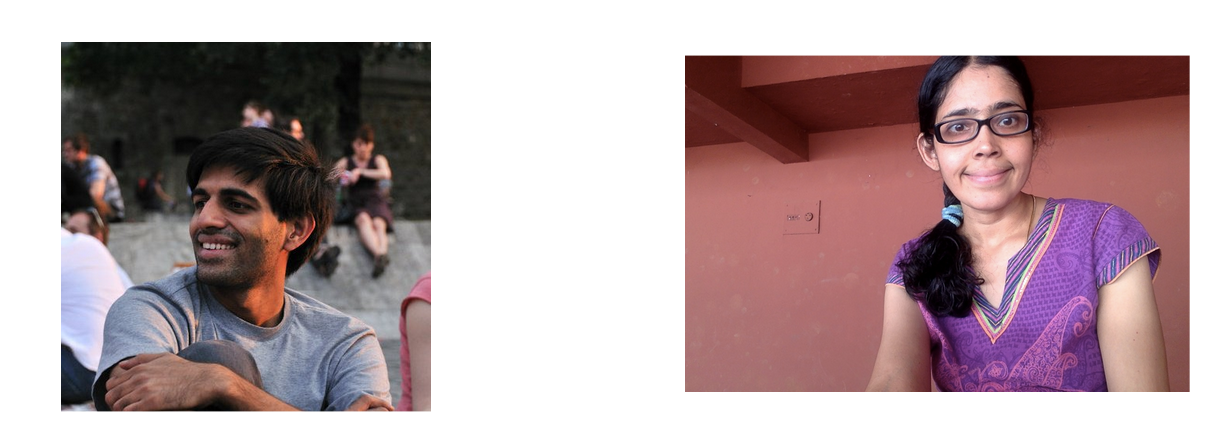
\includegraphics[width=\textwidth]{fig/advisors.png}
% \end{frame}
% \begin{frame}{Thank You}
% \centering
% 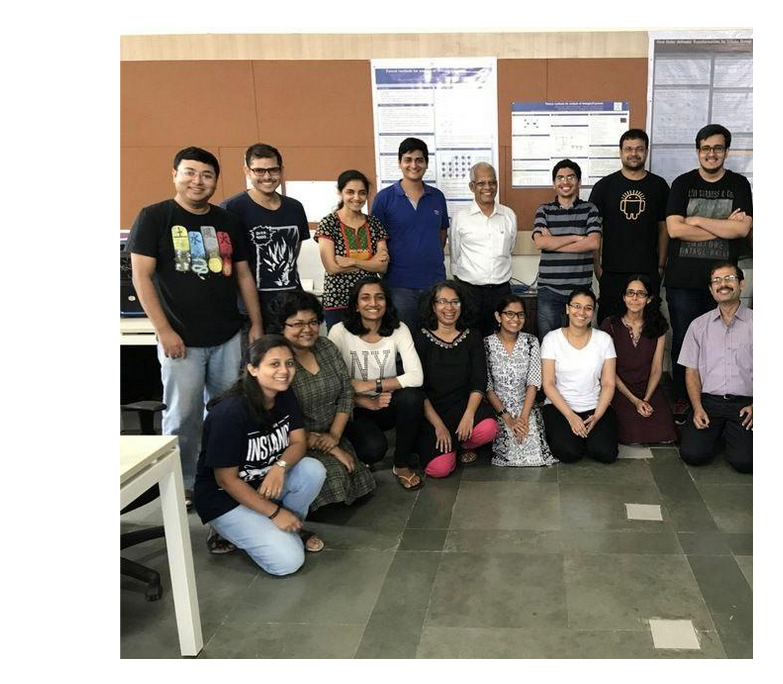
\includegraphics[width=\textwidth]{fig/labmates.png}
% \end{frame}
\begin{frame}
\begin{center}
     \LARGE{\textcolor{red}{Questions?}}
     \end{center}
   \end{frame}
   %%%%%%%%%%%%%%%%%%%%%%%%%5
    \begin{frame}[allowframebreaks]{Bibliography}
 
       \bibliographystyle{plainnat}
   {\tiny \bibliography{biblio}}

 \end{frame}
 %%%%%%%%%%%%%%%
%  \begin{frame}{Untimed $\forall$-Resilience is EXPSPACE-C}
%   \begin{itemize}
%     \item A timed automata $\ta$ is not untimed $\forall$-resilient if and
%       only if there is a faulty run that is not untimed-BTN
%       \item One can construct a product automaton  with state space
%         $ \region{\faultyta}\times 2^{\region{\ta}}\times [-1,K] $
%         \begin{itemize}
%         \item Synchronizes only after $K$ steps after the fault
%         \item State space is double exponential thus, can be solved in EXPSPACE
%           \end{itemize}
%       \end{itemize}
%       \pause
%       \begin{block}{Hardness:}
%         The hardness comes from the untimed language inclusion of
%         timed automata
%         \end{block}
% \end{frame}

% %%%%%%%%%%%%%%%%%%%%%%%%%%%%%%%%%
%  %%%%%%%%%%% 5
% \begin{frame}{Untimed $\exists$-Resilience is PSPACE-C}
%   \begin{itemize}
%     \item Let $q = (l,r)$ be a state of $\region{\faultyta}$ reached
%       after a just faulty run.
%   \item One can non-deterministically guess in PSPACE a state of $\region{\ta}$
%     such that, there exists an
%    accepting run with same suffix as an accepting run from $q$ after
%    $K$ steps
%  \item Checking if a run is accepting  is in PSPACE
   
%   \end{itemize}
%   \pause
%   \begin{block}{Hardness:}
%     The hardness comes from the emptiness problem of timed automata
%     \end{block}
%   \end{frame}
%   %%%%%%%%%%%%%%%%%%%%5
%  % \subsection{Timed Resilience}
%   %%%%%%%%%%%%%%%%%%%%%%%%%
%   \begin{frame}{Why Timed Resilience is Difficult?}
%     \begin{itemize}
%     \item The number of just-faulty runs are infinite,
     
%         \item Can not use region automata directly as we need exact
%           timings 
%       \end{itemize}
%     \end{frame}
% \begin{frame}{$\forall$-Resilience is Undecidable!}
%   Reduction from timed automata language inclusion problem.
%     \pause
% \begin{figure}[t]
%   \begin{center}
%   \resizebox{\textwidth}{!}{
% \begin{tikzpicture}[shorten >=1pt,node distance=4cm,on grid,auto] 
% \begin{scope}
%   \node[state,initial] (b_0) {$s_0$};
%   % \node (dot_1)[above=of b_0,xshift=-.5cm] {};
%   % \node (dot_2)[below=of b_0,xshift=-.5cm] {};
%   % \node (dot_3) [right=of dot_1,xshift=5cm] {};
%   % \node (dot_4) [right=of dot_2,xshift=5cm] {};
%   % \draw[dashed] (dot_1) -- (dot_2);
%   % \draw[dashed] (dot_3) -- (dot_4);
%   % \draw[dashed] (dot_1) -- (dot_3);
%   % \draw[dashed] (dot_2) -- (dot_4);
%   \node[state] (b_1) [ right=of b_0] {$s_i$}; \node[state] (b_2)
%   [above right=of b_1,yshift=-1.2cm] {$s_{i,1}$}; \node[state] (b_3)
%   [below right=of b_1,yshift=1.2cm] {$s_{i,2}$}; \node[state]
%   (l_{0,1}) [right of=b_2] {$s_1$}; \node[state] (l_{0,2}) [right
%   of=b_3] {$s_2$};

%   \path[-latex] (b_0) edge node {$x \leq 10,a,\{y\}$} (b_1){};
%   \path[-latex] (b_1) edge node {$x>11\wedge y<1,b,\emptyset$}
%   (b_2){}; \path[-latex] (b_1) edge node {$x\leq 10,b,\emptyset$}
%   (b_3){}; \path[-latex] (b_2) edge node {$z=15,c,X_1$} (l_{0,1}){};
%   \path[-latex] (b_3) edge node {$z=15,c,X_2$} (l_{0,2}){};
% \end{scope}
% \end{tikzpicture}
% }
% \end{center}

% \caption{The gadget automaton $\mathcal G_{und}$.}
% \label{fig:resil_time_undecidable}

% \end{figure}
% \end{frame}

% %%%%%%%%%%%%%% 5
% \begin{frame}{$\exists$-Resilience is in EXPSPACE}
%   Let us define a product automaton $\faultyta \bigotimes_{K} \ta$ with state space,
%   $L_{\faultyta} \times L_{\ta} \times [-1,K] \times
%   V:(X_{\faultyta}\cup X_{\ta})\rightarrow \mathbb{R}_{\geq 0}$
%   \pause
%   \begin{itemize}
%     \item The transitions will synchronize time till $K$ steps of the
%       fault
%     \item Then it will synchronize on actions and time both.
%       \item Accepts when both reach acceptance condition
%       \end{itemize}
% \pause
%       % \begin{textblock*}{5cm}(5cm,5.6cm) % {block width} (coords) 
%       %   {\scriptsize
% \textcolor{blue}{Given a run $\rho^{\otimes}$ of $\faultyta
%   \bigotimes_{K} \ta$, projection to the first component of
%   $\rho^{\otimes}$ is a run of $\faultyta$}


% % \end{textblock*}
%   \end{frame}
%   %%%%%%%%%%%%%% 5
% \begin{frame}{$\exists$-Resilience is in EXPSPACE}

%   Let $\rho_f$ be a faulty accepting run of $\ta_{\faultmod}$.  
%   \begin{center}
%     \pause
%   $\rho_f$ is BTN in $K$-steps
%   \pause
  
%   \textcolor{red}{$\Updownarrow$}
%   \pause
  
%  there is an accepting run $\rho^{\otimes}$ of
%     $\ta_{\faultmod} \otimes_K \ta$ s.t. the \textcolor{blue}{projection} on its
%     first component is $\rho_{f}$
%   \end{center}
%   \pause
%   For a given run $\rho_f$ there are \emph{infinitely} many runs
%   $\rho^{\otimes}$ of $\ta_{\faultmod} \otimes_K \ta$ for infinitely
%   many runs $\rho_i$ of $\ta$.
  
%   \pause
%   If we use $\region{\ta_{\faultmod} \otimes_K \ta}$, we
%   will loose the information that the runs $\rho_f$ and $\rho_i$ have
%   equal duration.
%   % \pause
%   %    \textcolor{red}{$\region{\faultyta \bigotimes_{K} \ta$} is  not
%   %      enough because even
% \end{frame}
% %%%%%%%%%%%%%%%%%%
% \begin{frame}{Strong Region automata}
%   Given a timed automata $\mathcal{B}$ we construct strong($\mathcal{B}$) by adding,
%   \begin{itemize}
%   \item A virtual clock $x_\iota$ that resets in each global time
%   \item $x_\iota < 1$ constraint to each transitions
%     \item virtual self loop to each locations with guard $x_\iota = 1$
%       resetting $x_\iota$
%     \end{itemize}
%     We call $\region{strong(\mathcal{B})}$  the strong region automata
%     of $\mathcal{B}$.
%   \end{frame}
%   %%%%%%%%%%%%%%%%%%%%%%%%
%     \begin{frame}{Strong Construction Example}
%       \begin{figure}[t]
%         \scalebox{0.7}{
%     \begin{tikzpicture}[]
%       \node[initial above,cir,initial text={}] at (0,0) (A1) {$s_1$} ;
%       \node[cir] at (2,0) (B1) {$s_2$}; \node[cir1,accepting] at (5,0)
%       (C1) {$s_3$}; \draw [-latex] (A1) edge node [midway,above]
%       {\scriptsize$t_1, y<1$} node[midway,below]{\scriptsize $z:=0$} (B1); \draw [-latex] (B1) edge node
%       [midway,above] {\scriptsize$ t_4,1<y< 2\wedge z<1$} (C1); \draw
%       [-latex] (B1) edge [loop below] node [below]
%       {\scriptsize$t_2,y:=0$} (B1); \draw [-latex] (B1) edge
%       [out=300,in=330,looseness=8] node [right]
%       {\scriptsize$t_3,z:=0$} (B1);
%     \end{tikzpicture}}
%   \scalebox{0.7}{
%      \begin{tikzpicture}
%       \node[initial above,cir,initial text={}] at (0,0) (A1) {$s_1$} ;
%       \node[cir] at (3,0) (B1) {$s_2$}; \node[cir1,accepting] at (7,0)
%       (C1) {$s_3$}; \draw [-latex] (A1) edge node [midway,above]
%       {\scriptsize$ t_1,y<1,z:=0$} node [near start,below]
%       {\scriptsize$ \strongclock<1$}(B1); \draw [-latex] (B1) edge node
%       [midway,above] {\scriptsize$t_4, 1<y< 2\wedge z<1$} node [near
%       end,below] {\scriptsize$ \strongclock<1$} (C1); \draw [-latex] (A1) edge
%       [loop below] node [below] {\scriptsize$ \strongclock=1,\strongclock:=0$} (A1); \draw
%       [-latex] (C1) edge [loop below] node [below]
%       {\scriptsize$ \strongclock=1,\strongclock:=0$} (C1); \draw [-latex] (B1) edge [loop
%       below] node [below] {\scriptsize$ \strongclock=1,\strongclock:=0$} (B1); \draw
%       [-latex] (B1) edge [out=100,in=130,looseness=8] node [above ]
%       {\scriptsize$t_2,\strongclock<1,y:=0$} (B1); \draw [-latex] (B1) edge
%       [out=300,in=330,looseness=8] node [right]
%       {\scriptsize$t_3,\strongclock<1,z:=0$} (B1);
%     \end{tikzpicture}
%  }
%   \caption{Example timed automaton  and  its strong timed
%     automaton}\label{fig:example-ta}
% \end{figure}

% % {\scriptsize $\sigma = (s_1,[\{0\},\{0\}]) \overset{t_1}\longrightarrow
% % (s_2,[(0,1),\{0\}]) \overset{t_2}\longrightarrow (s_2,[\{0\},(0,1)])
% % \overset{t_3}\longrightarrow (s_2,[(0,1),\{0\}])
% % \overset{t_4}\longrightarrow (s_3,[(1,2),(0,1), \fpart{y}<
% % \fpart{z}])$.}

% {\scriptsize
%   $\rho_1=(t_1,d_1=0.8)(t_2,d_2=1.2)(t_3,d_3=1.9)(t_4,d_4=2.4)$}

% {\scriptsize $\rho_2=(t_1,d'_1=0.9) (t_2,d'_2=1.89)
%   (t_3,d'_3=2.69)(t_4,d'_4=3.39)$}

% \pause

% {\scriptsize But, $\fpart{d_2} < \fpart{d_3}$ but $\fpart{d'_2} > \fpart{d'_3}$.}
%   \end{frame}
%   %%%%%%%%%%%%%%%%%
% % \begin{frame}{$\exists$-Resilience is in EXPSPACE}
% %   Assume two runs  of $\ta$
  
% %   $\rho_{1} = (t_{1},d_{1}),(t_{2},d_{2})\cdots$
  
% %   $\rho_{2} = (\tau_{1},e_{1}),(\tau_{2},e_{2})\cdots$
  
% %   \pause
% %   \begin{center}
% %   $\rho_{1} \sim_{\rho} \rho_{2}$ iff,
% %   \begin{itemize}
% %   \item $\abs{\rho_{1}} = \abs{\rho_{2}}$
% %   \item $t_{i} = \tau_{i}, \mbox{ for all } i$
% %   \item $\lfloor d_{i}\rfloor = \lfloor e_{i} \rfloor$ for all $i$
% %     \end{itemize}
% %   \end{center}
% %   \pause
% %   \textcolor{red}{The relation $\sim_{\rho}$ is an equivalence
% %     relation of finite index}
% % \end{frame}
% %%%%%%%%%%%%%%%%%

%   \begin{frame}{$\exists$-Resilience is in EXPSPACE}
%     For a given just faulty run $\rho_{f}$ we define,
%     \begin{itemize}[<+->]
%       \item $T_{\rho_{f}}^{\otimes_{K}}=
%         \{(l_{\faultyta},l_{\ta},K,\nu) \mid
%         (l_{\faultyta},l_{\ta},K,\nu) \mbox{ is a state of } \faultyta
%         \bigotimes_{K} \ta\mbox{ reachable by following } \rho_{f}^{\otimes}$\}
%         \item $S^{\otimes_{K}}_{\rho_{f}} =
%           \{(l_{\faultyta},l_{\ta},K,r) \in \region{\faultyta
%         \bigotimes_{K} \ta} \mid (l_{\faultyta},l_{\ta},K,\nu) \in
%       T_{\rho_{f}}^{\otimes_{K}} \mbox{ and } \nu \models r\} $
%     \end{itemize}
   
    
% \pause
% \begin{block}{Safeness}
%     $S^{\otimes_{K}}_{\rho_{f}}$ is safe if we can reach an accepting state of $\region{\faultyta
%         \bigotimes_{K} \ta}$ from a state
%       $(l_{\faultyta},l_{\ta},K,r)$ in
%       $S^{\otimes_{K}}_{\rho_{f}}$
%       \end{block}
%     \end{frame}
  
% %%%%%%%%%%%%%% 5
% \begin{frame}{$\exists$-Resilience is in EXPSPACE}
% For two just faulty runs $\rho_{1}$ and $\rho_{2}$, that follow same
% path in the strong region automata of $\faultyta$,

% \begin{itemize}
% \item We show that $S^{\bigotimes_{K}}_{\rho_{1}} =
%   S^{\bigotimes_{K}}_{\rho_{2}}$ (via re-timing)
%   \item We can enumerate all possible  $S^{\bigotimes_{K}}_{\rho}$
%     in EXPSPACE
%     \item Checking if $ S^{\bigotimes_{K}}_{\rho}$ is safe can be
%       done in PSPACE
   
%     \end{itemize}
%     \pause
% Hence, $\exists$-resilience is in \textcolor{red}{EXPSPACE}

% \pause
% \begin{block}{Hardness}
%  We  show \textcolor{blue}{PSPACE} hardness by a reduction from
%  emptiness of timed automata
%  \end{block}
% \end{frame}
% %%%%%%%%%%%%%55
                   
%                    \begin{frame}{Example}
%               \begin{figure}[ht]
%   \begin{center}
   
%       \begin{tikzpicture}[->,thick]
%       \node[initial below, cir1, initial text ={}] at (0,0) (A) {A} ; \node[cir1] at (4,0) (B) {B};
       
          
%         \path (A) edge node [above]{$x\leq 1, \textcolor{red}{0.2}$} node
%         [below]{$\set{x}$}(B);
%         \path(A) edge [loop above] node [above]{$x\leq 1, \textcolor{red}{0.8}$}(A);
%         \path(B) edge [loop right] node [right]{$x< 1,
%           \textcolor{red}{1}$}(B);
%         \path(B) edge [loop above] node [above]{$1\leq x\leq 2, \textcolor{red}{0.3}$}(B);
%                  \path (B)
%         edge[bend left] node [below]{$1 \leq x \leq 2,\textcolor{red}{0.7}$}(A);

          
       
%       \end{tikzpicture}\pause
%       \vspace{1cm}
%        \begin{tikzpicture}[->,thick]
%       \node[initial below, dia, initial text ={}] at (0,0) (A) {A} ; \node[dia] at (4,0) (B) {B};
%       \node[cir] at (2,1) (C) {C};
%       \node[cir] at (2,-1) (D) {D};
       
          
%         \path (C) edge[bend left] node [above]{$\top,
%           \textcolor{red}{2}$} node[below,xshift=-10,yshift=5]{$\set{x}$}
%        (B);
%         \path (A) edge[bend right] node [below]{$x\leq 1$}(C);
%         \path(C) edge[bend right]  node [above]{$\top, \textcolor{red}{8}$}(A);
%         \path(B) edge [loop right] node [right]{$x< 1$}(B);
%         \path(B) edge [bend left] node [right,xshift=3]{$1\leq x\leq 2$}(D);
%         \path(D) edge [bend left] node [above]{ $\top$,\textcolor{red}{3}}(B);
%                  \path (D)
%         edge[bend left] node [below]{$\top,\textcolor{red}{7}$}(A);

        
%       \end{tikzpicture}
 
%     \label{fig:ex2}
%   \end{center}
% \end{figure}

% \end{frame}

%%%%%%%%%%%% 5
\section{Algorithm and Tool for Hole Bounded Reachability of \mpda}
\begin{frame}{Decidability \& Some Possible Algorithms}
  \begin{theorem}
The $K$-hole bounded reachability of \mpda{} is decidable
   \end{theorem}
   \begin{itemize}[<+->]
   \item Hole bounded $\Rightarrow$ Tree-width bounded
     \item Tree-width bounded $\Rightarrow$ Decidable reachability~\cite{madhusudan2011tree}
   \end{itemize}
   
   \pause
  \begin{itemize}[<+->]
  \item Tree-width based Algorithm~\cite{AkshayGKS17},
    \begin{enumerate}
    \item Capture the behaviour of the model as a graph
    \item Show that these graphs has bounded tree-width
    \item Solve Reachability using Tree-automata
      
    \end{enumerate}
    \pause
  \hspace{6cm} \begin{rotate}{30}\textcolor{red}{Difficult to design!}
        \end{rotate}
  \item Naive BFS exploration
      
    \begin{enumerate}
    \item makes arbitrary nondeterministic choices  
      \end{enumerate}
      \pause
  \hspace{6cm} \begin{rotate}{30}\textcolor{red}{Unnecessary branches!}
        \end{rotate}  
  \end{itemize}
  
\end{frame}
\end{document}
%%%%%%%%%%%%%%%%%%%%5
    
%%% Local Variables:
%%% mode: latex
%%% TeX-master: t
%%% End:
      

